\NeedsTeXFormat{LaTeX2e}
\documentclass[a4paper,12pt,
headsepline,           % Linie zw. Kopfzeile und Text
oneside,               % einseitig
pointlessnumbers,      % keine Punkte nach den letzten Ziffern in Überschriften
bibtotoc,              % LV im IV
%DIV=15,               % Satzspiegel auf 15er Raster, schmalere Ränder   
BCOR15mm               % Bindekorrektur
%,draft
]{scrbook}
\KOMAoptions{DIV=last} % Neuberechnung Satzspiegel nach Laden von Paket helvet

\pagestyle{headings}
\usepackage{blindtext}

\usepackage{algorithm}
\usepackage{algpseudocode}

% für Texte in deutscher Sprache
\usepackage[english]{babel}
\usepackage[utf8]{inputenc}
\usepackage[T1]{fontenc}

% Helvetica als Standard-Dokumentschrift
\usepackage[scaled]{helvet}
\renewcommand{\familydefault}{\sfdefault} 

\usepackage{graphicx}
\usepackage{subcaption}

% Literaturverzeichnis mit BibLaTeX
% \usepackage[babel,german=quotes]{csquotes}
\usepackage[style=english]{csquotes}
\usepackage[backend=bibtex8]{biblatex}
\bibliography{bibliography}

% Alternative mit Paket-Option backend=biber und \addbibresource
% \usepackage[backend=biber]{biblatex}

% \addbibresource{bibliography.bib}

% Für Tabellen mit fester Gesamtbreite und variabler Spaltenbreite
\usepackage{tabularx} 

% Besondere Schriftauszeichnungen
\usepackage{url}              % \url{http://...} in Schreibmaschinenschrift
\usepackage{color}            % zum Setzen farbigen Textes

\usepackage{amssymb,amsmath,amsthm} % Pakete für Mathe-Umgebungen und -Symbole
\setcounter{MaxMatrixCols}{20}

\usepackage{todonotes}

\usepackage{algorithm}
\usepackage{algpseudocode}

\usepackage{setspace}         % Paket für div. Abstände, z.B. ZA
%\onehalfspacing              % nur dann, wenn gefordert; ist sehr groß!!
\setlength{\parindent}{0pt}   % kein linker Einzug der ersten Absatzzeile
\setlength{\parskip}{1.4ex plus 0.35ex minus 0.3ex} % Absatzabstand, leicht variabel

% Tiefe, bis zu der Überschriften in das Inhaltsverzeichnis kommen
\setcounter{tocdepth}{3}      % ist Standard

% Beispiele für Quellcode
\usepackage{listings}
\lstset{language=Java,
  showstringspaces=false,
  frame=single,
  numbers=left,
  basicstyle=\ttfamily,
  numberstyle=\tiny}

% hier Namen etc. einsetzen
\newcommand{\fullname}{Ilja Sukhanov}
\newcommand{\email}{ilja.sukhanov@uni-ulm.de}
\newcommand{\titel}{Spectral Scale Selection for Kernel Density Estimation}
\newcommand{\jahr}{2026}
\newcommand{\matnr}{1211998}
\newcommand{\gutachterA}{Prof.\,Dr.\,Evgeny Spodarev}
\newcommand{\gutachterB}{Prof.\,Dr.\,Henning Bruhn-Fujimoto}

% hier die Fakultät auswählen
%\newcommand{\fakultaet}{---  Im Quellcode anpassen nicht vergessen! ---}
\newcommand{\fakultaet}{Mathematik und\\Wirtschafts-\\wissenschaften}

% hier das Institut einsetzen
\newcommand{\institut}{Institut für Stochastik}

% Informationen, die LaTeX in die PDF-Datei schreibt
\pdfinfo{
  /Author (\fullname)
  /Title (\titel)
  /Producer     (pdfeTex 3.14159-1.30.6-2.2)
  /Keywords ()
}

\usepackage{amsfonts}
\usepackage{mathtools}
\usepackage{booktabs}
\usepackage{hyperref}
\hypersetup{
pdftitle=\titel,
pdfauthor=\fullname,
pdfsubject={Diplomarbeit},
pdfproducer={pdfeTex 3.14159-1.30.6-2.2},
colorlinks=false,
pdfborder=0 0 0	% keine Box um die Links!
}

% Trennungsregeln
\hyphenation{Sil-ben-trenn-ung}


\newtheorem{Def}{Definition}
\newtheorem{Prop}{Proposition}
\newtheorem{Thm}{Theorem}
\newtheorem{Example}{Example}
\newtheorem{Lem}{Lemma}
\newtheorem{Rem}{Remark}
\newtheorem{Cor}{Corollary}
\newtheorem{conjecture}{Conjecture}


\begin{document}
\frontmatter

% Titelseite
\thispagestyle{empty}
\begin{addmargin*}[4mm]{-10mm}

\hfill

\includegraphics[height=1.8cm]{Abschlussarbeit_2021/LaTeX/images/logo_uulm_sw.pdf}\\[1em]

{\footnotesize
%{\bfseries Universität Ulm} \textbar ~89069 Ulm \textbar ~Germany
\hspace*{115mm}\parbox[t]{35mm}{\bfseries Fakultät für\\
\fakultaet\\
% TODO hier Institut anpassen
\mdseries \institut}\\[2cm]

\parbox{140mm}{\bfseries \LARGE \titel}\\[2.5em]
{\footnotesize Abschlussarbeit an der Universität Ulm}\\[3em]

{\footnotesize \bfseries Vorgelegt von:}\\
{\footnotesize \fullname\\ \email}\\ \matnr\\[2em]
{\footnotesize \bfseries Gutachter:}\\                     
{\footnotesize \gutachterA\\ \gutachterB}\\[2em]
% {\footnotesize \bfseries Betreuer:}\\ 
% {\footnotesize \betreuer}\\\\
{\footnotesize \jahr}
}
\end{addmargin*}


% Impressum
\clearpage
\thispagestyle{empty}
{ \small
  \flushleft
  Fassung \today \\\vfill
  \copyright~\jahr~\fullname\\[0.5em]
% Wenn Sie Ihre Arbeit unter einer freien Lizenz bereitstellen möchten, können Sie die nächste Zeile in Ihren Code aufnehmen. Bitte beachten Sie, dass Sie hierfür an allen Inhalten, inklusive enthaltener Abbildungen, die notwendigen Rechte benötigen! Beim Veröffentlichungsexemplar Ihrer Dissertation achten Sie bitte darauf, dass der Lizenztext nicht den Angaben in den Metadaten der genutzten Publikationsplattform widerspricht. Nähere Information zu den Creative Commons Lizenzen erhalten Sie hier: https://creativecommons.org/licenses/
%This work is licensed under the Creative Commons Attribution 4.0 International (CC BY 4.0) License. To view a copy of this license, visit \href{https://creativecommons.org/licenses/by/4.0/}{https://creativecommons.org/licenses/by/4.0/} or send a letter to Creative Commons, 543 Howard Street, 5th Floor, San Francisco, California, 94105, USA. \\
  Satz: PDF-\LaTeXe
}

% ab hier Zeilenabstand etwas größer 
\setstretch{1.2}

\tableofcontents

\mainmatter
\chapter*{Abstract}

\todo[inline]{Write abstract (150-250 words)}
\chapter{Introduction and Methodology}\label{chap:intro_meth}

How can one choose a meaningful scale from a multiscale family of statistical objects?



\section{Simplicial Complexes}

We begin by introducing the simplicial complex, the main mathematical object in Topological Data Analysis. For literature consult \cite{Dey_Wang_2022}.

\begin{Def}[Abstract simplicial complex]
    Let $V$ be a finite set of vertices. An abstract simplicial complex $K$ is a collection of subsets of $V$ such that:
    \begin{itemize}
        \item $\emptyset\in K$
        \item $\{v\}\in K$ for every $v\in V$
        \item if $\sigma\in K$ and $\tau\subseteq\sigma$ then $\tau\in K$
    \end{itemize}
    We denote by $\mathcal{K}(V)$ the set of all simplicial complexes with vertex set $V$.
\end{Def}

An element $\sigma\in K$ is called face. The dimension of a face $\sigma$ is $\dim{\sigma}=|\sigma|-1$. The dimension of $K$ is $\dim{K}=\max\{\dim{\sigma}:\sigma\in K\}$. A face $\sigma\in K$ with $\dim{\sigma}=\dim{K}$ is called facet.

Note that a simplicial complex $K$ with $\dim{K}=1$ is a simple graph. Thus, an abstract simplicial complex can be considered as a generalization of a simple graph.

The abstract simplicial complex is a purely combinatorial object. It can be given a geometric meaning by embedding it in the $d$-dimensional euclidean space.

\begin{Def}[Geometric realization]
    The geometric realization of an abstract simplicial complex $K$ with vertex set $V=\{v_1,\dots,v_n\}$ is given by
    \begin{align*}
        |K|_{\Phi}=\bigcup\limits_{\sigma\in K}\operatorname{conv}\{p_t:t\in\sigma\},
    \end{align*}
    where $\Phi:V\to\mathbb{R}^m$ is an embedding map that may have further properties.
\end{Def}

\todo[inline]{Geometric volume depends on the embedding.}

\todo[inline]{$2d+1$ theorem}

Using the geometric realization $|K|_{\Phi}$ the volume of a simplex $\sigma=[v_{i_0}\dots v_{i_j}]$ can be defined by
\begin{align*}
    \operatorname{Vol}(\sigma):= \frac{1}{j!}\sqrt{\det{\left(\langle x_{i_k}-x_{i_0},x_{i_l}-x_{i_0}\rangle_{k,l=1}^{j}\right)}},
\end{align*}
where $\langle x_k,x_l\rangle_{k,l=1}^{j}$ is the Gram matrix defined by $X^TX$ with $X=(x_1\cdots x_j)$. We see that $\operatorname{Vol}(\sigma)=0$ for all $\sigma\in K$ with $\dim{\sigma}<\dim{K}$. The volume of a simplicial complex is
\begin{align*}
    \operatorname{Vol}(K)=\sum_{\sigma\in K,\dim{\sigma}=\dim{K}}\operatorname{Vol}(\sigma)
\end{align*}

\subsection*{Binary operations on simplicial complexes}

\todo[inline]{Symmetric difference}

There exist different operations $\oplus:\mathcal{K}(V)\times\mathcal{K}(V)\to\mathcal{K}(V)$ which we will discuss below. The union of two complexes $K_1$ and $K_2$ is defined as
\begin{align*}
    K_1\cup K_2:=\{\sigma\subseteq V:\sigma\in K_1\text{ or }\sigma\in K_2\}
\end{align*}

\todo[inline]{Give general discussion on operations $\oplus\in\{\cup,\dots\}$ with examples}

\section{Topological Data Analysis}

\todo[inline]{Cite papers about TDA intro}

Let $(V,\Sigma)$ be an abstract simplicial complex and denote by $\Sigma_k$ the set of all simplices in $\Sigma$ with dimension $k$. Let $C_k(\mathbb{F})$ be the free Abelian group generated using $\Sigma_k$ as the basis with linear coefficients from the field $\mathbb{F}$, that is,
\begin{align*}
    C_k(\mathbb{F})=\left\{\sum_{i=1}^{n}k_i\sigma_i:\sigma_i\in\Sigma_K,k_i\in\mathbb{F},n\in\mathbb{N},i=1,\dots,n\right\}.
\end{align*}
Throughout this work, we will only consider $\mathbb{F}=\mathbb{Z}_2=\{0,1\}$ and set $C_k(\mathbb{Z}_2)=C_k$. The sum in [] is seen as a formal sum: the coefficient $k_i=0$ means that the simplex $\sigma_i$ is excluded and the coefficient $k_i=1$ means that the simplex $\sigma_i$ is included in the sum. Next we define the boundary map $\delta_k:\Sigma_k\to C_{k-1}$ by
\begin{align*}
    \delta_k(\sigma):=\sum_{i=0}^{k}(-1)^{i}\sigma_{-i},\quad\sigma=[x_0\dots x_k]\in\Sigma_k,
\end{align*}
where $\sigma_{-i}\in\Sigma_{k-1}$ is the simplicial complex with vertices $x_0,\dots,x_{i-1},x_{i+1},\dots,x_k$. We extend $\delta_k$ from $\Sigma_k$ to $C_k$ by the rule
\begin{align*}
    \delta_k(\Gamma):=\sum_{i=1}^{n}k_i\delta_k(\sigma_i),
\end{align*}
where $\Gamma=\sum_{i=1}^{n}k_i\sigma_i\in C_k$.

The $k$-th Betti number $\beta_k$ is set to be the dimension of the image of $\delta_k$:
\begin{align*}
    \beta_k=\dim(\operatorname{Im}\delta_k)
\end{align*}

\section{Methodology}

\begin{itemize}
    \item Mutual information, information theory:
    \begin{align*}
        I(X,Y)=H(X)+H(Y)-H(X,Y)
    \end{align*}
    where $H$ is the entropy (measure of complexity)
    \item Green matrix, Min-/Meet-matrix
    \item do multiple samples and see if critical $\epsilon$ changes (stability under resampling)
\end{itemize}

For two simplicial complexes $K_1$ and $K_2$, we define the $f$-based divergence as
\begin{align*}
    \langle K_1,K_2\rangle_f&:=f(K_1)+f(K_2)-f(K_1\oplus K_2),
\end{align*}
where $f$ is any nonnegative integer-valued (subadditive) function defined on simplicial complexes. For example $f(K)=\text{cat}(K)$. Due to the subadditivity of $f$, the scalar product is nonnegative. A stronger notion would be submodularity. Then it would hold $\left\langle K_1,K_2\right\rangle_f\ge f(K_1\cap K_2)\ge0$.

\todo[inline]{add discussion about $\langle K_1,K_2\rangle_f=0\iff$??}

For a finite sequence of filtration values $\epsilon_1,\dots,\epsilon_N$ we can define a matrix $\Sigma^{(N)}=(\Sigma^{(N)}_{ij})$ by
\begin{align*}
    \Sigma^{(N)}_{ij}:=\left\langle K_{\epsilon_i}(X),K_{\epsilon_j}(X)\right\rangle_f,\quad i,j=1,\dots,N.
\end{align*}
Since we consider a filtration $K_{\epsilon_1}\subseteq\dots\subseteq K_{\epsilon_{N}}$, the scalar product is just given by $\left\langle K_{\epsilon_i},K_{\epsilon_j}\right\rangle_f=f(K_{\epsilon_i}\cap K_{\epsilon_j})=f(K_{\epsilon_{i\wedge j}})$, where $i\wedge j:=\min\{i,j\}$. This means that the subadditivity of $f$ is not needed for the nonnegativity of the scalar product when considering a filtration. Setting $c_i=f(K_{\epsilon_i})$, the scale similarity matrix has the following form:
\begin{align}\label{eq:Sigma_form}
    \Sigma^{(N)}=\begin{pmatrix}
        c_1 & c_1 & \dots & c_1\\
        c_1 & c_2 & \dots & c_2\\
        \vdots & \vdots & \ddots & \vdots\\
        c_1 & c_2 & \dots & c_N
    \end{pmatrix}
\end{align}

The following lemma shows that the local extrema of the vector $c=(c_1,\dots,c_N)$ and the principal eigenvector $v^*$ of $\Sigma^{(N)}$ coincide. In particular, choosing a functional $f$ such that $i\mapsto f(K_{\epsilon_i})$ is monotone might not be a good idea, since the entries of the principal eigenvector will merely reflect the monotone behavior of $f$. This suggests that we need to choose a functional $f$ such that $i\mapsto f(K_{\epsilon_i})$ is non-monotone.

% The following lemma shows that using the $\min$ kernel might not be a good idea, as we do not gain any advantages from computing the principal eigenvector $v^*$ of $\Sigma^{(N)}$. Concretely, the entries of any eigenvector of $\Sigma^{(N)}$ have the same behavior as the map $i\mapsto f(K_{{\epsilon_i}})$.

\begin{Lem}
    Let $\Sigma\in\mathbb{R}^{N\times N}$ be defined by $\Sigma_{ij}=f(K_{\epsilon_{i\wedge j}})$ and denote $c_i:=f(K_{\epsilon_i})$ for $i=1,\dots,N$. Then for the principal eigenvector $v$ of $\Sigma$ it holds that
    \begin{align*}
        \operatorname{sgn}(v_{i+1}-v_i)=\operatorname{sgn}(c_{i+1}-c_i),\quad\forall i=1,\dots,N-1.
    \end{align*}
\end{Lem}
\begin{proof}
    Let $\lambda$ be the largest eigenvalue of $\Sigma$ with corresponding (principal) eigenvector $v$. Then $\Sigma v=\lambda v$. By Perron-Frobenius $\lambda>0$. We remember that the matrix $\Sigma$ has the form~\eqref{eq:Sigma_form} and compute
    \begin{align*}
        \lambda(v_{i+1}-v_i)&=\lambda v_{i+1}-\lambda v_i\\&
        =(\Sigma v)_{i+1}-(\Sigma v)_i\\&
        =\left(c_1v_1+\dots+c_{i}v_{i}+c_{i+1}\sum_{l=i+1}^{N}v_l\right)\\&-\left(c_1v_1+\dots+c_{i-1}v_{i-1}+c_i\sum_{l=i}^{N}v_l\right)\\&
        =c_{i+1}\sum_{l=i+1}^{N}v_l-c_i\sum_{l=i+1}^{N}v_l\\&
        =(c_{i+1}-c_i)\sum_{l=i+1}^{N}v_l.
    \end{align*}
    Since by Perron-Frobenius all entries of $v$ are positive, we have $\sum_{l=i+1}^{N}v_l>0$ in addition to $\lambda>0$. It follows that $\text{sgn}(v_{i+1}-v_i)=\text{sgn}(c_{i+1}-c_i)$ which is the claim.
\end{proof}

An interesting question arises concerning the global extrema of $c$ and $v^*$. Do they coincide as well? If not, how would counterexamples look like?
\todo[inline]{add discussion about global extrema}

\begin{Prop}[Properties of the Min-matrix]\label{prop:properties_of_min_matrix}
    Let $\Sigma=(\Sigma_{ij})\in\mathbb{R}^{N\times N}$ with $\Sigma_{ij}=\min\{c_i,c_j\}$ for some constants $c_1,\dots,c_N\in\mathbb{R}_{\ge0}$.
    \begin{enumerate}
        \item[1.] $\Sigma$ is positive semi-definite iff $0\le c_1\le\dots\le c_N$
        \item[2.] $\Sigma$ is positive definite iff $0<c_1<\dots<c_N$
        \item[3.] The determinant of $\Sigma$ is given by $\operatorname{det}(\Sigma)=c_1(c_2-c_1)\cdots(c_N-c_{N-1})$
        \item[4.] The inverse of $\Sigma$ exists iff $c_{i+1}-c_{i}\ne0$ for all $i=1,\dots,N-1$ and is given by $\Sigma^{-1}=(\Sigma^{-1}_{ij})$ with
        \begin{align*}
            \Sigma^{-1}_{ii}&=\begin{cases}
                \frac{1}{c_i-c_{i-1}}+\frac{1}{c_{i+1}-c_i} & ,i=1,\dots,N-1\\
                \frac{1}{c_{N}-c_{N-1}} & ,i=N
            \end{cases}\\
            \Sigma^{-1}_{i,i+1}&=\Sigma^{-1}_{i+1,i}=-\frac{1}{c_{i+1}-c_i},i=1,\dots,N-1
        \end{align*}
    \end{enumerate}
\end{Prop}
\begin{proof}
    \todo[inline]{Prove in appendix or cite}
\end{proof}

% Question: under which conditions on $f$ is $\Sigma$ positive definite or positive semi-definite

\begin{Rem}
    From Proposition~\ref{prop:properties_of_min_matrix} it follows that the scale similarity matrix $\Sigma$ is positive definite iff $i\mapsto f(K_{\epsilon_i})$ is monotonously strictly increasing and positive.
\end{Rem}

A matrix $\Sigma=(\Sigma_{ij})\in\mathbb{R}^{N\times N}$ is called nonnegative (positive) if $\Sigma_{ij}\ge0$ ($\Sigma_{ij}>0$) for all $i,j=1,\dots,N$. It is called primitive if it is nonnegative and there exists a natural number $m$ such that $\Sigma^{m}$ is positive. The spectrum $\sigma(\Sigma)$ is the (multi-)set of all eigenvalues of $\Sigma$: $\sigma(\Sigma)=\{\lambda\in\mathbb{C}:\exists v\in\mathbb{C}^N,v\ne0:\Sigma v=\lambda v\}$.

\todo[inline]{add definition of irreducible matrix}
\todo[inline]{discuss conditions on matrices}

% \todo[inline]{algebraic multiplicity = 1 $\implies$ geometric multiplicity = 1 $\implies$ eigenvector is unique up to scaling}

\begin{Thm}[Perron-Frobenius]
    Let $\Sigma=(\Sigma_{ij})\in\mathbb{R}^{N\times N}$ be a primitive matrix. Then there exist $\lambda^*>0$ and $v^*=(v^*_1,\dots,v^*_N)\in\mathbb{R}^{N}_{>0}$ such that $\lambda^*\in\sigma(\Sigma)$, $\lambda^*>|\lambda|$ for all $\lambda\in\sigma(\Sigma),\lambda\ne\lambda^*$. Furthermore, $v^*$ is the corresponding eigenvector that is unique up to scaling.
\end{Thm}

\begin{Rem}
    Analogously to classical PCA, we can study the spectral gap ratio: $\frac{\lambda_N-|\lambda_N|}{\lambda_N}$
\end{Rem}

\subsubsection*{critical scale choice}

We are now interested in $j_{\text{crit}}=\text{argmax}_{j=1,\dots,N}\{v^{\star}_j\}$. We pick $\epsilon_{\text{crit}}=\epsilon_{j_{\text{crit}}}$ and consider all vertices that are isolated in $\text{VR}_{\epsilon_{\text{crit}}}(X)$ as noise.

\todo[inline]{Discuss uniqueness of $j_{\text{crit}}$}

\subsubsection*{Connection to Markov Chains}

\todo[inline]{Doob $h$-transform}

Let $\Sigma_N$ be the scale similarity matrix with principal eigenvector $v^*=(v^*_1,\dots,v^*_N)$ and corresponding eigenvalue $\lambda^*$. Let $\{1,\dots,N\}$ be the state space and introduce the transition matrix
\begin{align*}
    P=\frac{1}{\lambda^*}D_{v^*}^{-1}\Sigma_ND_{v^*},
\end{align*}
where $D_{v^*}=\operatorname{diag}(v^*_1,\dots,v^*_N)$. The resulting Markov chain is reversible and ergodic. Its stationary distribution $\pi=(\pi_1,\dots,\pi_N)$ is given by
\begin{align*}
    \pi_j=\frac{v^*_j}{\sum_{k=1}^{N}(v^*_k)^2}
\end{align*}

\begin{Rem}
    The Donsker-Varadhan free-energy functional $\mathcal{F}$ is known to be
    \begin{align*}
        \mathcal{F}_{\Sigma}(Q)=\sum_{i,j=1}^{N}\pi_i^{Q}q_{ij}\log{\left(\frac{\Sigma_{ij}}{q_{ij}}\right)}
    \end{align*}
    where $Q=(q_{ij})$ is any positive, row-stochastic matrix with stationary distribution $\pi^{Q}$. It holds $\mathcal{F}(Q)\le\mathcal{F}(P)$ for any positive, row-stochastic matrix $Q$, where $P$ is the matrix introduced in Equation~[]. This fact serves as motivation for the replacement of our initial scale similarity matrix $\Sigma_N$ with the transition matrix $P$: we replace $\Sigma_N$ which is non-stochastic by the closest (in the above sense) stochastic matrix $P$.
\end{Rem}

\section{Monotone scale selection}

\todo[inline]{implement a function in Python that computes the stationary birth death distribution}

We consider the case $0<c_1<\dots<c_N$. Define the discrete Laplacian:
\begin{align*}
    \mathcal{L}=\frac{1}{c_1}\operatorname{diag}(1,0,\dots,0)-\Sigma^{-1}
\end{align*}
which acts as the generator of a birth-death chain on the state space $\{1,\dots,N\}$ with transition rates...

The normalized stationary distribution of the embedded birth-death chain is given by
\begin{align*}
    \pi^{\text{BD}}&=(\pi^{\text{BD}}_1,\dots,\pi^{\text{BD}}_N)\\
    \pi^{\text{BD}}_j&=\frac{r_j}{\overline{r}}\\
    r_j&=\begin{cases}
        \frac{1}{c_2-c_1}, & j=1\\
        \frac{1}{c_j-c_{j-1}}+\frac{1}{c_{j+1}-{c_j}}, & j=2,\dots,N-1\\
        \frac{1}{c_N-c_{N-1}}, & j=N
    \end{cases}\\
    \overline{r}&=\sum_{j=1}^{N}r_j
\end{align*}

The critical scales are naturally identified as
\begin{align*}
    j_{\text{crit}}\in\arg\min\{\pi^{\text{BD}}_j:j=1,\dots,N\}
\end{align*}

\section{Other combinatorial and topological features of simplicial complexes}

In this section we present and discuss function defined on simplicial complexes that are non-negative, integer valued and sub-additive. Let $\mathcal{F}(K)$ denote the set of all facets of $K$, i.e. all simplices $\sigma\in K$ with $\dim\sigma=\dim K$.

\textbf{$f$-vector.} The $f$-vector of a simplicial complex $K$ is $f(K)=(f_0,f_1,\dots,f_d)$, where $f_k$, $k=-1,0,\dots,d$ is the number of simplices in $K$ containing $k+1$ vertices. Using the $f$-vector, we can construct the $f$-polynomial:
\begin{align*}
    F_K(t)=\sum_{k=-1}^{d}f_kt^{k+1}=1+f_0t+f_1t^2+\dots+f_dt^{d+1}
\end{align*}

\textbf{Betti numbers.} Informally speaking, the $k$-th Betti number $\beta_k(K)$ of a simplicial complex $K$ represents the number of $k$-dimensional holes. In particular, $\beta_0(K)$ is the number of connected components of $K$. We could also consider the total Betti number (the sum of all Betti numbers): $\sum_{k}\beta_k(K)$.

\textbf{Euler characteristic.} The Euler characteristic is given by
\todo[inline]{motivation, proof}
\begin{align*}
    \chi(K)=\sum_{k=0}^{d}(-1)^{k}f_k(K)=\sum_{k=0}^{d}(-1)^{k}\beta_k(K)
\end{align*}

\textbf{Vertex cover number.} The vertex cover number is defined as
\begin{align*}
    \tau(K):=\min\{|C|:C\subseteq V(K),C\cap F\ne\emptyset\forall F\in\mathcal{F}(K)\}
\end{align*}

\textbf{Matching number.} The matching number is defined as
\begin{align*}
    \nu(K):=\max\{|M|:M\subseteq\mathcal{F}(K),F\cap F'=\emptyset\forall F,F'\in M, F\ne F'\}
\end{align*}

The matching number can be computed using the blossom algorithm.

\textbf{Chain count.} The chain count of length $r\in\mathbb{N}$ is defined as
\begin{align*}
    c_r(K):=|\{(\sigma_0\nsubseteq\sigma_1\nsubseteq\dots\nsubseteq\sigma_r):\sigma_i\in K\}|
\end{align*}

\textbf{Degree-type counts.} The degree-type counts of dimension $t\in\mathbb{N}_0$ are defined as
\begin{align*}
    \Delta_t(K):=\max_{\tau\in K}|\{\sigma\in K:\tau\subseteq\sigma,\dim\sigma=t\}|
\end{align*}

% \begin{itemize}
%     \item graph based descriptors of the 1-skeleton (graph-theoretic invariants): vertex cover number, number of connected components, arboricity, minimum spanning tree
%     \item general construction?
%     \item instead of $f$ vector count $k$ simplexes that are not part of $k+1$ simplexes
%     \item integer linear programming?
%     \item use persistence diagrams (distance between persistence diagrams), bar codes, birth and death intervals to construct matrix (persistence landscape norm, persistence entropy)
%     \item $n_k(\epsilon)=\#\{(b,d)\in\text{PD}_k:b\le\epsilon<d\}$ or $L_k(\epsilon)=\sum_{(b,d)\in\text{PD}_k,b\le\epsilon<d}(d-b)$
% \end{itemize}

\begin{Rem}
    Here we discuss how the functionals presented above simplify when the sampled points live on a line $\mathbb{R}^1$. Then there is only the $0$-th Betti number $\beta_0$ (the number of connected components). The $f$-vector only has one non-trivial component: the number of edges $f_1$.
\end{Rem}


We consider the following general form of the functional:
\begin{align*}
    f(K)=f_{\text{Top}}(K)\cdot f_{\text{Comb}}(K),
\end{align*}
where the topological part $f_{\text{Top}}$ is defined by
% \begin{align*}
%     f_{\text{Top}}(K)=\delta_{-1}+\sum_{j=0}^{d-1}\delta_j\beta_j^{\alpha_j}(K)+\delta_d\operatorname{cup}_R^{\alpha_d}(K)+\delta_{d+1}\operatorname{PC}^{\alpha_{d+1}}(K)
% \end{align*}
\begin{align*}
    f_{\text{Top}}(K)=\delta_{-1}+\sum_{j=0}^{d-1}\delta_j\beta_j^{\alpha_j}(K)
\end{align*}
with coefficients $\delta_j\in\mathbb{R}$, $j=-1,0,\dots,d-1$ and $\alpha_j\in\mathbb{R}$, $j=0,\dots,d-1$. The combinatorial part $f_{\text{Comb}}$ is defined by
% \begin{align*}
%     f_{\text{Comb}}(K)&=\gamma_{-1}+\sum_{j=0}^{d}\gamma_jf_j^{\xi_j}(K)+\gamma_{d+1}\operatorname{CR}_{k,m}^{\xi_{d+1}}(K)+\gamma_{d+2}c_r^{\xi_{d+2}}(K)\\&
%     +\gamma_{d+3}\Delta_t^{\xi_{d+3}}(K)+\gamma_{d+4}\tau^{\xi_{d+4}}(K)+\gamma_{d+5}\nu^{\xi_{d+5}}(K)
% \end{align*}
\begin{align*}
    f_{\text{Comb}}(K)&=\gamma_{-1}+\sum_{j=0}^{d}\gamma_jf_j^{\xi_j}(K)
\end{align*}
with coefficients $\gamma_j\in\mathbb{R}$, $j=-1,0,\dots,d$ and $\xi_{j}\in\mathbb{R}$, $j=0,\dots,d$.

This function serves as a building kit that lets us construct a polynomial-type combination of all the features that we introduced earlier. For example, setting $\delta_0=1$, $\delta_j=0$ for $j\ne 0$, $\gamma_1=1$, $\gamma_j=0$ for $j\ne1$ and $\alpha_j=\xi_j=1$ recovers the product $\beta_0f_1$ which is the number of edges $f_1$ multiplied by the number of connected components $\beta_0$ (see \cite{leonov-report}). If we consider a filtration $K_{\epsilon}$, then if $\epsilon$ increases, $f_1$ increases (more edges appear), but $\beta_0$ decreases (connected components merge), so this is a non-monotone kind of functional.

\todo[inline]{Talk about how to recover the Euler characteristic using this functional}


\begin{Def}
    A triple $(f,\{K_i\},\oplus)$ is said to be spectrally optimizable if it generates a finite irreducible discrete time Markov chain on the state space $\{1,\dots,N\}$ with transition probability matrix $Q=(q_{ij})$ and stationary distribution $\pi^Q=(\pi_1^Q,\dots,\pi_N^Q)$.
\end{Def}

\todo[inline]{Is there an alternative MC construction that favors \enquote{kink points}?}

\todo[inline]{Stationary distribution construction for asymmetric scale similarity matrices}

\section{General methodology beyond complexes}

Above we have considered a sequence (filtration) of simplicial complexes $K_{\epsilon_i}$, $0<\epsilon_1<\dots<\epsilon_N$ and have constructed a similarity/ mutual information using a functional $f(K)$ by
\begin{align*}
    \langle K_1,K_2\rangle_f=f(K_1)+f(K_2)-f(K_1\oplus K_2)
\end{align*}
where $\oplus$ is some combining operation.

How can we generalize this beyond complexes? For example for a sequence of kde's $f_{h_i}$, $0<h_1<\dots<h_N$ or a sequence of point clouds $\mathcal{P}_k\subseteq\mathbb{R}^{k}$, $k=1,\dots,k_{\max}$?
% \chapter{Application to ARMA processes}

The application of TDA to time series analysis is well established (\cite{perea_sliding_2015})\todo{cite papers about TDA for time series}. A prominent example that shows the connection between these two fields clearly are (noisy) sine curves: at the right scale, the two dimensional sliding window reveals a loop. See \cite{KARAN2021115326}

In the first section, we give an overview on the theory of time series needed for our purposes. Next we discuss the embedding of time series as point clouds in $\mathbb{R}^k$, where Takens' theorem will play an important role. Finally, we present our numerical results and interpret them.

\todo[inline]{Main Question: Sequence of what?}

\todo[inline]{TDA and Sliding window embedding not even needed?}

\todo[inline]{Main goal: Prove consistency of spectrally selected order $k^{\star}$ to the true order $p$}

\section{Preliminaries on time series}

For information on autoregressive moving-average (ARMA) models, see Brockwell et al~\cite[Chapter~3]{brockwell2016introduction}. 

We consider a family of random variables $(Z_t)_{t\in\mathbb{Z}}$ that has the following properties:
\begin{subequations}\label{eq:white-noise-assumptions}
    \begin{align}
        \mathbb{E}[Z_t] &= 0,
        && t\in\mathbb{Z}, \label{eq:white-noise-centered}\\
        \operatorname{Var}[Z_t] &= \sigma^2\in(0,+\infty),
        && t\in\mathbb{Z}, \label{eq:white-noise-variance}\\
        \operatorname{Cov}[Z_t,Z_s] &= 0,
        && t,s\in\mathbb{Z},\ t\neq s. \label{eq:white-noise-uncorrelated}
    \end{align}
\end{subequations}

Later, we will drop the finite variance assumption~\eqref{eq:white-noise-variance} and replace the uncorrelated assumption~\eqref{eq:white-noise-uncorrelated} with independence.

For the innovations $Z_t$, we will consider the following distributions:
\begin{itemize}
    \item Uniform: $Z_t\sim\mathcal{U}[-a,a]$ for some $a>0$ (variance: $\operatorname{Var}[Z_t]=a^2/3$)
    \item Normal: $Z_t\sim\mathcal{N}(0,\sigma^2)$
    \item Student-t: $Z_t\sim t_{\nu}$ for some degrees of freedom $\nu>0$ (the variance does not exist for $\nu\le2$)
\end{itemize}

The last distribution is part of a more general kind of distributions that fulfills
\begin{align*}
    \mathbb{P}(|Z|>x)=x^{-\alpha}L(x)
\end{align*}
for some $\alpha\in(0,2)$ and a slowly varying function $L$. 

\todo[inline]{establish hierarchy: alpha stable, slowly varying property, heavy tails}

Some common heavy tailed distributions are
\begin{itemize}
    \item Cauchy: $X\sim C(x_0,\gamma)$
    \item Levy: $X\sim L()$
    \item Pareto: $X\sim P()$
    \item Student-t: $X\sim t_{\nu}$
\end{itemize}

\begin{Def}
    Let $(Z_t)_{t\in\mathbb{Z}}$ be a family of random variables satisfying the assumptions~\eqref{eq:white-noise-assumptions}. A process $(X_t)$ is an ARMA($p$, $q$) process if
    \begin{align}\label{eq:def_arma}
        X_t=\sum_{i=1}^{p}\phi_iX_{t-i}+Z_t+\sum_{j=1}^{q}\theta_jZ_{t-j}, && t\in\mathbb{Z},
    \end{align}
    where the polynomials $\phi(z):=1-\phi_1z-\dots-\phi_pz^{p}$ and $\theta(z):=1+\theta_1z+\dots+\theta_qz^{q}$ are required to have no common factors. Additionally, $\phi_p\neq0$ and $\theta_q\neq0$.
\end{Def}

In case of $\theta\equiv1$ we recover the autoregressive (AR) process of order $p\in\mathbb{N}$ and $X_t$ has the form
\begin{align}\label{eq:ar(p)}
    X_t=\sum_{i=1}^{p}\phi_iX_{t-i}+Z_t,
\end{align}
where $\phi_i\in\mathbb{R}$ are the coefficients with $\phi_p\ne0$.

It is well known that there exists a stationary process $(X_t)_{t\in\mathbb{Z}}$ that can be written in the form \eqref{eq:def_arma} if $\phi(z)\neq0$ for all $z\in\mathbb{C},\lvert z\rvert=1$. Another important property that we will need for the geometric interpretation of the embedded AR process is causality: An ARMA process $(X_t)$ is called causal if there exist constants $\psi_j$ with $\sum_j|\psi_j|<+\infty$, such that $X_t=\sum_{j=0}^{\infty}\psi_jZ_{t-j}$ for all $t\in\mathbb{Z}$. It turns out that this property is stronger than stationarity, as an ARMA process is causal iff $\phi(z)\neq0$ for all $z\in\mathbb{C},\lvert z\rvert\le1$. In what follows, we will exclusively work with causal ARMA processes.

For our experiments, we use random coefficients $\theta_1,\dots,\theta_q\sim\mathcal{U}[-1,1]$ since there are no restrictions on these coefficients for the ARMA process to be causal. For the AR coefficients, we will first draw $\phi'_1,\dots,\phi'_p\sim\mathcal{U}[-1,1]$ and then set $\phi_i=\text{sc}\cdot\phi_i'/\|\phi'\|_1$ for some scale parameter $\text{sc}<1$. This is a necessary condition for the generated AR($p$) processes to be causal.

\todo[inline]{Find sufficient condition implementation}

\todo[inline]{Discuss automatic coefficient selection}

\section{Order selection methods}

There are several established methods for choosing an order $\hat{p}$ given a realization $X=(X_1,\dots,X_T)$ that is assumed to come from an AR($p$) process. 

\begin{itemize}
    \item Final Prediction Error (FPE) Criterion
    \item Akaike Information Criterion (AIC)
    \item Bayesian Information Criterion (BIC)
\end{itemize}

\todo[inline]{Are there any guarantees for the quality of such selectors?}

\todo[inline]{order selection for heavy tailed innovations? Look for papers}

Once the order has been chosen, the AR coefficients $\phi_1,\dots,\phi_{\hat{p}}$ can be estimated using one of the following classical procedures:
\begin{itemize}
    \item Yule-Walker Estimation
    \item Burg's Algorithm
    \item The Hannan-Rissanen Algorithm
    \item Maximum Likelihood Estimation
\end{itemize}



\section{Embedding of time series}

In order to apply machinery from Topological Data Analysis to time series data, one has to embed the time series into $\mathbb{R}^k$ for some embedding dimension $k\in\mathbb{N}$. The main method for this is the so called sliding-window embedding (see~\cite{perea_sliding_2015}), which we will describe in detail now. Let $X=(X_1,\dots,X_T)$ be one realization of some univariate time series. Then we obtain a point cloud from $X$ by defining:
\begin{align*}
    Y_t^{(k)}&=\begin{pmatrix}
        X_{t}\\
        X_{t+1}\\
        \vdots\\
        X_{t+k-1}
    \end{pmatrix}\in\mathbb{R}^k\\ 
    \mathcal{P}_{k}&=\left\{Y_t^{(k)}:t=1,\dots,T-k_{\max}+1\right\}\subseteq\mathbb{R}^k
\end{align*}
Here, $k\in\mathbb{N}$ is the dimensionality of the point cloud $\mathcal{P}_{k}$ and $k_{\max}$ a predetermined upper cap, that is, $k\in\{1,\dots,k_{\max}\}$.

\todo[inline]{Give discussion why it does not matter if we consider the past or future $k$ observations for the geometry of the point cloud (forward versus backward embedding)}

Takens' Theorem mainly serves as a theoretical justification or motivation for the sliding-window embedding.

\begin{Thm}[Takens]
    Let $\mathcal{M}$ be a compact manifold of dimension $m$. Let $\phi\in\operatorname{Diff}^2(\mathcal{M})$ and $y\in C^2(\mathcal{M},\mathbb{R})$. Then the map $\Phi_{(\phi,y)}:\mathcal{M}\to\mathbb{R}^{2m+1}$ defined by
    \begin{align*}
        \Phi_{(\phi,y)}(x)=\begin{pmatrix}
            y(x)\\
            y(\phi(x))\\
            \vdots\\
            y(\phi^{2m}(x))
        \end{pmatrix}
    \end{align*}
    is an embedding, given that the pair $(\phi,y)$ is generic.
\end{Thm}

\todo[inline]{connect Takens' Theorem better, add interpretation}

\todo[inline]{study time dynamics, formation of loops, $t$ vs number of loops until $t$, size of loops (how many time steps before loop closes)}

\section{Scale Selection for the AR-process application}

Consider the sequence of point clouds $\mathcal{P}_k$ with increasing dimension $k\in\mathbb{N}$. Our goal is to apply the scale selection principle presented in Chapter~\ref{chap:methodology} to determine an \enquote{optimal} scale $k^{\star}\in\{1,\dots,k_{\max}\}$. In order to apply the scale selection, we need to construct a sequence (not necessarily a filtration) of simplicial complexes $\{L_k\}_{k=1}^{k_{\max}}$. Afterwards, we need to choose what kind of operation $\oplus$ we use to combine the simplicial complexes and the right type of functional (preferably of topological nature) to evaluate the simplicial complexes. In the end, we want to find a triple $(f,\{K_k\}_{k=1}^{k_{\max}},\oplus)$ that is spectrally optimizable.

\enquote{Optimality} of $k^{\star}$ should encompass $k^{\star}=p$ or at least $k^{\star}\approx p$ where the meaning of $\approx$ is specified. In particular, this \enquote{optimal} scale selection serves as an order estimation method without requiring the existence of (second) moments of the innovations.

\subsection*{Dimension lift}

The first step is to lift the point clouds $\mathcal{P}_k$, $k=1,\dots,k_{\max}$ to a common ambient dimension. That is, transforming each $\mathcal{P}_k$ to $\mathcal{Q}_k\subseteq\mathcal{R}^{k_{\max}}$. In order to do this, we split the observed time series $X=(X_1,\dots,X_T)$ into a train and test part:
\begin{align*}
    X_{\text{train}}&=(X_1,\dots,X_{T'})\\
    X_{\text{test}}&=(X_{T'+1},\dots,X_T)
\end{align*}

For $k\in\{1,\dots,k_{\max}\}$ we complete $Y_{t}^{(k)}=(X_t,X_{t+1},\dots,X_{t+k-1})^{T}\in\mathbb{R}^{k}$ to
\begin{align*}
    p_{t}^{(k)}&=\begin{pmatrix}
        I_k\\
        \hat{A}_k
    \end{pmatrix}Y_t^{(k)}=\begin{pmatrix}
        Y_{t}^{(k)}\\
        \hat{A}_kY_{t}^{(k)}
    \end{pmatrix}\\
    &=\begin{pmatrix}
        X_t\\
        X_{t+1}\\
        \vdots\\
        X_{t+k-1}\\
        \hat{\alpha}_{1,1}^{(k)}X_t+\dots+\hat{\alpha}_{1,k}^{(k)}X_{t+k-1}\\
        \vdots\\
        \hat{\alpha}_{k_{\max}-k,1}^{(k)}X_{t}+\dots+\hat{\alpha}_{k_{\max}-k,k}^{(k)}X_{t+k-1}
    \end{pmatrix}\in\mathbb{R}^{k_{\max}},\\
    t&=T'+1,\dots,T-k_{\max}+1,
\end{align*}
where $I_k\in\mathbb{R}^{k\times k}$ is the identity matrix and $\hat{A}_k\in\mathbb{R}^{(k_{\max}-k)\times k}$ a linear completion matrix with coefficients $\hat{\alpha}_{i,j}^{(k)}$, $i=1,\dots,k_{\max}-k$, $j=1,\dots,k$. The completed part $\hat{A}_kY_{t}^{(k)}$ resembles $z_t^{(k)}=(X_{t+k},\dots,X_{t+k_{\max}-1})^{T}\in\mathbb{R}^{k_{\max}-k}$ (the next $k_{\max}-k$ observations after $Y_t^{(k)}$).

We determine $\hat{A}_k$ by minimizing a functional $\Psi_k(A_k)$ that depends on the train data $X_{\text{train}}$. The kind of functional depends on the nature of the innovation distribution. For example, we might choose different $\Psi_k$ depending on whether the innovations are light tailed or heavy tailed. Afterwards, we set $\hat{z}_t^{k}=\hat{A}_kY_{t}^{(k)}$ and $p_t^{k}=(Y_{t}^{(k)},\hat{z}_t^{k})$. We denote the lifted point cloud by $\mathcal{Q}_k=\{p_t^{k}:t=k_{\max},\dots,T\}$.


We are interested in the geometry of the point cloud $\mathcal{Q}_k$. We write
\begin{align*}
    p_t^{(k)}&=\sum_{j=1}^{k}X_{t-j+1}\cdot h_j, & h_j=\begin{pmatrix}
        e_j\\
        \hat{\alpha}_{1,j}\\
        \vdots\\
        \hat{\alpha}_{k_{\max}-k,j}
    \end{pmatrix},
\end{align*}
where $e_j$ is the $j$-th unit vector in $\mathbb{R}^{k}$. Note that the directions $h_1,\dots,h_k$ are independent of $t$. Therefore, $\mathcal{Q}_k$ is contained in a $k$-dimensional linear subspace of $\mathbb{R}^{k_{\max}}$, namely $\operatorname{span}\{h_1,\dots,h_k\}$.

Note that we have the following equation:
\begin{align}\label{eq:squared_2norm_of_lifted_points}
    \left(p_t^{(k)}-p_s^{(k)}\right)^{T}\left(p_t^{(k)}-p_s^{(k)}\right)&=\left(Y_t^{(k)}-Y_s^{(k)}\right)^{T}\left(I_k+\hat{A}_k^{T}\hat{A}_k\right)\left(Y_t^{(k)}-Y_s^{(k)}\right).
\end{align}
% Linear completion changes metric according to how strongly observed coordinates predict missing coordinates

We have
\begin{align*}
    M_t^{(k)}\cdot\begin{pmatrix}
        X_T\\
        \vdots\\
        X_1
    \end{pmatrix}=
    p_t^{(k)},
\end{align*}
where the matrix $M_t^{(k)}\in\mathbb{R}^{k_{\max}\times T}$ is given by
\begin{align*}
    \begin{pmatrix}
        \mathbf{0} & I_k & \mathbf{0}\\
        \mathbf{0} & \hat{A}_k & \mathbf{0}
    \end{pmatrix},
\end{align*}
with $\mathbf{0}$ being matrices of the right size that contain only zeros.

\subsubsection*{Dimension lift via Least Squares (Light tailed case)}

In case of light tailed innovations, we can determine the linear completion matrix by Ordinary Least Squares (see the book~\cite{Grey_1981} for information on OLS with a vector valued response). That is, we determine
\begin{align}\label{eq:ls_dimension_lift}
    \hat{A}_k\in\arg\min\left\{\sum_{t=1}^{T'-k_{\max}+1}\left\|z_t^{(k)}-AY_{t}^{(k)}\right\|_2^2:A\in\mathbb{R}^{(k_{\max}-k)\times k}\right\}.
\end{align}
The Problem~\eqref{eq:ls_dimension_lift} can be formulated in a more compact way using matrix notation. To this end, we introduce the matrices
\begin{align*}
    Y_k&=\begin{pmatrix}
        Y_{1}^{(k)} & \cdots & Y_{T'-k_{\max}+1}^{(k)}
    \end{pmatrix}\in\mathbb{R}^{k\times(T'-k_{\max}+1)}\\
    Z_k&=\begin{pmatrix}
        z_{1}^{(k)} & \cdots & z_{T'-k_{\max}+1}^{(k)}
    \end{pmatrix}\in\mathbb{R}^{(k_{\max}-k)\times(T'-k_{\max}+1)}
\end{align*}
and Problem~\eqref{eq:ls_dimension_lift} becomes
\begin{align*}
    \hat{A}_k\in\arg\min\left\{\operatorname{tr}\left((Z_k-AY_k)^{T}(Z_k-AY_k)\right):A\in\mathbb{R}^{(k_{\max}-k)\times k}\right\}.
\end{align*}



The solution can be written down explicitly:
\begin{align*}
    \hat{A}_k&=Z_kY_k^{T}\left(Y_kY_k^{T}\right)^{-1}\\&
    =\underbrace{\sum_{t=1}^{T'-k_{\max}+1}z_t^{(k)}\left(Y_t^{(k)}\right)^T}_{=U_k}\left(\underbrace{\sum_{t=1}^{T'-k_{\max}+1}Y_t^{(k)}\left(Y_t^{(k)}\right)^{T}}_{=V_k}\right)^{-1},
\end{align*}
provided that $V_k=Y_kY_k^{T}$ is invertible. This is almost surely the case if the innovations have an absolute continuous distribution.

\todo[inline]{Prove $\mathbb{P}(Y_kY_k^{T}\text{ is invertible})=1$ explicitly}

% cite Mityagin

The entries of the matrices $U_k=(U_{ij}^{(k)})\in\mathbb{R}^{(k_{\max}-k)\times k}$ and $V_k=(V_{ij}^{(k)})\in\mathbb{R}^{k\times k}$ can be written as
\begin{align*}
    U_{ij}^{(k)}&=\sum_{t=1}^{T'-k_{\max}+1}X_{t+k+i-1}X_{t+j-1},\quad i=1,\dots,k_{\max}-k,j=1,\dots,k\\
    V_{ij}^{(k)}&=\sum_{t=1}^{T'-k_{\max}+1}X_{t+i-1}X_{t+j-1},\quad i,j=1,\dots,k
\end{align*}
By the ergodic theorem (??) these entries converge and their limit is determined by the auto-covariance function $\gamma$ of the process $(X_t)$:
\begin{align*}
    \tilde{U}_{ij}^{(k)}&=\frac{1}{T-k_{\max}+1}U_{ij}^{(k)}\stackrel{T\to\infty}{\to}\mathbb{E}\left[X_{t+k+i-1}X_{t+j-1}\right]=\gamma(j-i-k)\\
    \tilde{V}_{ij}^{(k)}&=\frac{1}{T-k_{\max}+1}V_{ij}^{(k)}\stackrel{T\to\infty}{\to}\mathbb{E}\left[X_{t+i-1}X_{t+j-1}\right]=\gamma(j-i)
\end{align*}
Thus we have the following convergence, which is understood component wise:
\begin{align*}
    \hat{A}_k=U_kV_k^{-1}\stackrel{T\to\infty}{\to}\operatorname{Cov}\left[z_t^{(k)},Y_t^{(k)}\right]\left(\operatorname{Cov}\left[Y_t^{(k)}\right]\right)^{-1}.
\end{align*}


The uncompleted part $z_t^{(k)}$ can be expressed as a linear function of $Y_t^{(k)}$ and innovations $Z=(Z_{t+k},\dots,Z_{t+k_{\max}-1})$ \textcolor{red}{once $k\ge p$}. That is, there exist matrices $B_k$ and $C_k$ such that $z_t^{(k)}=B_kY_t^{(k)}+C_kZ$. This is not surprising because linearity is already part of the AR process. Thus, our linear prediction $\hat{z}_t^{(k)}=\hat{A}_kY_t^{(k)}$ is a natural choice.

The matrices $B_k$ and $C_k$ can be determined by first writing
\begin{align*}
    &H_k\begin{pmatrix}
        Y_{t}^{(k)}\\
        z_t^{(k)}
    \end{pmatrix}=\begin{pmatrix}
        Z_{t+k}\\
        \vdots\\
        Z_{t+k_{\max}-1}
    \end{pmatrix}\\&
    z_t^{(k)}=-H_z^{-1}H_YY_t^{(k)}-H_z^{-1}\begin{pmatrix}
        Z_{t+k}\\
        \vdots\\
        Z_{t+k_{\max}-1}
    \end{pmatrix}
\end{align*}
with
\begin{align*}
    H_k=\begin{pmatrix}
        0 & \cdots & 0 & \phi_p & \phi_{p-1} & \cdots & \phi_1 & 1 & 0 & \cdots & 0\\
        0 & \cdots & 0 & 0 & \phi_p & \phi_{p-1} & \cdots & \phi_1 & 1 & \cdots & 0\\
        \vdots & & \vdots & \vdots & \ddots & \ddots & \ddots & & \ddots & \ddots & \vdots\\
        0 & \cdots & 0 & 0 & \cdots & 0 & \phi_p & \phi_{p-1} & \cdots & \phi_1 & 1
    \end{pmatrix}
\end{align*}
and reconstruction matrix $B_k=-H_z^{-1}H_Y$, where $H_p^{(k)}=(H_Y H_z)$. Note that $H_z$ is in fact invertible since it is a lower triangular matrix with all diagonal elements being equal to $1$.

\todo[inline]{What about a representation in the case $k<p$}

\subsubsection*{Dimension lift via Excursion metric minimization}

\begin{itemize}
    \item $F_0\sim X_t$? Take empirical cdf
    \item When is $X_t$ ergodic?
\end{itemize}

We again have an observed time series $X=(X_{1},\dots,X_T)$ that is split up into $X_{\text{train}}=(X_1,\dots,X_{T_{\text{train}}})$ and $X_{\text{test}}=(X_{T_{\text{train}}+1},\dots,X_T)$. Define $X^{\text{test}}_t=X_{T_{\text{train}}+t}$ for $t=1,\dots,T-T_{\text{train}}$. The goal is to lift $Y_t^{(k)}$ for $t=T_{\text{train}}+1,\dots,T$ from $\mathbb{R}^k$ to $\mathbb{R}^{k_{\max}}$. Denote the lifted point by $p_t^{(k)}$. It is given by
\begin{align*}
    p_t^{(k)}=\begin{pmatrix}
        X_{t}\\
        X_{t+1}\\
        \vdots\\
        X_{t+k-1}\\
        \hat{X}_{t+k}\\
        \vdots\\
        \hat{X}_{t+k_{\max}-1}
    \end{pmatrix}
\end{align*}
with
\begin{align*}
    \hat{X}_{t+k-1+m}=\sum_{j=1}^{k}\lambda_j^{(m)}X_{t+j-1}, && m=1,\dots,k_{\max}-k
\end{align*}
The coeficients $\lambda_j^{(m)}$ are determined by
\begin{align*}
    \hat{\lambda}^{(m)}&\in\arg\min\left\{\mathcal{E}(X_{t+k-1+m},\hat{X}_{t+k-1+m})\right\}
\end{align*}
We have
\begin{align*}
    \mathcal{E}(X_{t+k-1+m},\hat{X}_{t+k-1+m})&=2\mathbb{E}\left[F(X_{t+k-1+m})\vee F(\hat{X}_{t+k-1+m})\right]\\&
    -\mathbb{E}\left[F(\hat{X}_{t+k-1+m})\right]-\frac{1}{2}
\end{align*}

The empirical version is
\begin{align*}
    \Phi(\lambda)&=\frac{2}{T_{\text{train}}-k_{\max}+1}\sum_{s=1}^{T_{\text{train}}-k_{\max}+1}F_{\hat{\theta}}\left(\sum_{j=1}^{k}\lambda_jX_{s-1+j}\right)\vee F_{\hat{\theta}}\left(X_{s+k-1+m}\right)\\&
    -\frac{2}{T_{\text{train}}-k_{\max}+1}\sum_{s=1}^{T_{\text{train}}-k_{\max}+1}F_{\hat{\theta}}\left(\sum_{j=1}^{k}\lambda_jX_{s-1+j}\right)-\frac{1}{2}
\end{align*}
where $F_{\hat{\theta}}$ is the empirical cumulative distribution function fitted on the data $X_{\text{train}}$.

\subsection*{Simplicial complex construction}

\begin{itemize}
    \item Temporal geometric complexes: $D_k(s,t)=\|Y_s^{(k)}-Y_t^{(k)}\|\le\epsilon_k$
    \item $E_k=\{\{s,t\}:D_k(s,t)\le\epsilon_k\}$, $\Sigma_{kl}=|E_k\cap E_l|$, $\Sigma_{kl}=|E_k\cap E_l|/|E_k\cup E_l|$
    \item $K_k=\operatorname{Flag}(V,E_k)$, $\Sigma_{kl}=f(K_k)+f(K_l)-f(K_k\cup K_l)$
    \item build $K_k$ from prediction errors, excursion distances or dependence scores
    \item $\oplus=\triangle$ (symmetric difference)
    \item $w_k(s,t)=d(\mathcal{L}(X_{s+k}|Y_s^{(k)}),\mathcal{L}(X_{t+k}|Y_t^{(k)}))$
\end{itemize}

\todo[inline]{give precedence: ordered temporal simplex, simplex generated by a directed path through time}

\todo[inline]{Does the clique closure performed by the flag complex preserve the information we care about? Many different weighted graphs can have exactly the same flag complex. We may actually lose information.}

A general construction principle can be described in a graph theoretical way. Consider the set of vertices $V=\{T_{\text{train}}+1,\dots,T-k_{\max}+1\}$. Two distinct time indices $s$ and $t$ form an edge if $w_k(s,t)\le\tau$, where $w_k:V\times V\to\mathbb{R}_{\ge0}$ is a weight function and $\tau>0$ some threshold parameter. Information about linear dependence enters via the choice of the weight function $w_k$. Let $E_k^{\tau}$ be the set of edges and $G_k^{\tau}=(V,E_k^{\tau})$ the resulting graph.

Now we take the flag complex $L_k^{\tau}=\text{Flag}(G_k^{\tau})$ and obtain a sequence of complexes $\{L_k^{\tau}\}_{k=1}^{k_{\max}}$. In order for $\{L_k\}_{k=1}^{k_{\max}}$ to be a filtration, it must hold
\begin{align*}
    w_{k+1}(e)\le w_{k}(e),&&\forall e\in E_k\text{ and }k=1,\dots,k_{\max}-1.
\end{align*}
At the moment, it is not clear whether the specific weighting choices discussed below fulfill this property.

The first candidate for $w_k$ is a norm of the covariance matrix. To this end, compute the covariance matrix:
\begin{align*}
    D_{s,t}^{(k)}=\operatorname{Cov}\left[p_t^{(k)},p_s^{(k)}\right]&=\begin{pmatrix}
        I_k\\
        \hat{A}_k
    \end{pmatrix}C_{s,t}^{(k)}\begin{pmatrix}
        I_k & \hat{A}_k^{T}
    \end{pmatrix}
\end{align*}

\begin{align*}
    C_{s,t}^{(k)}&=\operatorname{Cov}\left[Y_s^{(k)},Y_t^{(k)}\right]\\&=
    \begin{pmatrix}
        \mathbb{E}[X_sX_t] & \mathbb{E}[X_sX_{t+1}] & \cdots & \mathbb{E}[X_sX_{t+k-1}]\\
        \vdots & \vdots & & \vdots\\
        \mathbb{E}[X_{s+k-1}X_t] & \mathbb{E}[X_{s+k-1}X_{t+1}] & \cdots & \mathbb{E}[X_{s+k-1}X_{t+k-1}]
    \end{pmatrix}\\&
    =\begin{pmatrix}
        \gamma(s-t) & \gamma(s-t-1) & \cdots & \gamma(s-t-k+1)\\
        \gamma(s-t+1) & \gamma(s-t) & \cdots & \gamma(s-t-k+2)\\
        \vdots & \vdots & \ddots & \vdots\\
        \gamma(s-t+k-1) & \gamma(s-t+k-2) & \cdots & \gamma(s-t)
    \end{pmatrix}
\end{align*}

We need a scalar summary:
\begin{align*}
    &\rho_k(s,t)=\|C_{s,t}^{(k)}\|_F^2\\
    &\eta_k(s,t)=\|D_{s,t}^{(k)}\|_F^2=\left(k+\|\hat{A}_k\|_F^2\right)^2\|C_{s,t}^{(k)}\|_F^2
\end{align*}

\todo[inline]{autocovariance $\gamma(h)$ can be expressed via $\phi_1,\dots,\phi_p$ by using the Yule-Walker-Equations}

In cases where the second moment does not exist, the covariance is no longer viable. In such cases, we may use
\begin{align*}
    w_k(s,t)=\|p_s^{(k)}-p_t^{(k)}\|_1.
\end{align*}



\subsection*{Assembly of the scale similarity matrix}

We try out two different constructions:
\begin{align*}
    \langle L_i, L_j\rangle_f=f(L_i)+f(L_j)-f(L_i\cup L_j),
\end{align*}
where $f$ must be sub-additive, since $\{L_k\}_{k=1}^{k_{\max}}$ is not a filtration in general, and
\begin{align*}
    \langle L_i,L_j \rangle_f=f(L_i\cup L_j),
\end{align*}
where $f$ is non-negative. The scale similarity matrix becomes
\begin{align*}
    \Sigma_{k_{\max}}=\begin{pmatrix}
        \langle L_1, L_1\rangle_f & \langle L_1, L_2\rangle_f & \dots & \langle L_1, L_{k_{\max}}\rangle_f\\
        \langle L_1, L_2\rangle_f & \langle L_2, L_2\rangle_f & \cdots & \langle L_2, L_{k_{\max}}\rangle_f\\
        \vdots & \vdots & \ddots & \vdots\\
        \langle L_1, L_{k_{\max}}\rangle_f & \langle L_2, L_{k_{\max}}\rangle_f & \dots & \langle L_{k_{\max}}, L_{k_{\max}}\rangle_f
    \end{pmatrix}.
\end{align*}
Let $v^*=(v^*_1,\dots,v^*_{k_{\max}})$ be the principal eigenvector of $\Sigma_{k_{\max}}$. The \enquote{optimal} scale is set to $k^{*}\in\arg\max\{v^*_k:k=1,\dots,k_{\max}\}$.

\subsection*{Choice of the Functional $f$}

As a simple starting point, we try functionals of the form
\begin{align*}
    f(K)=\delta|C(K)|^{\alpha}|E(K)|^{\xi}
\end{align*}
or alternatively any transformation of $f$ that preserves monotonicity:
\begin{align*}
    \tilde{f}(K)&=\log{f(K)}=\tilde{\delta}+\alpha\log{\left(|C(K)|\right)}+\xi\log{\left(|E(K)|\right)}
\end{align*}

\todo[inline]{Some functional that measures the volume of the complex in some sense and detects the flatness}

\todo[inline]{graph functionals, mutual information from graph functionals}

\section{Statistical Approach}

\todo[inline]{Keep working on this idea!}

We obtain estimates of the coefficients and consider the error
\begin{align*}
    \hat{\sigma}_k^2=\frac{1}{n}\sum_{t}\left(X_t-\sum_{j=1}^{k}\hat{\alpha}_j^{(k)}X_{t-j}\right)
\end{align*}

Define the function $f$ on the class $\mathcal{A}_k(\mathcal{D})$ of all AR processes of order $k$ with innovations coming from the distribution $\mathcal{D}$ by
\begin{align*}
    f(\mathcal{A}_k(\mathcal{D}))=\frac{n}{2}\hat{\sigma}_k^{2}+\lambda k
\end{align*}



\section{Numerical Experiments}



Multiple questions arise:
\begin{itemize}
    \item How does increasing $k_{\max}$ influence the selection of $k^*$
    \item For fixed $k_{\max}$, $\alpha$, $\xi$ can $\tau$ be found such that the correct scale is chosen
    \item For fixed $\tau$ and $k_{\max}$ can $\alpha$ and $\xi$ be tuned?
\end{itemize}

\newpage

\section{Geometric Approach}

\todo[inline]{Explain why this idea is \enquote{dead}. Move to possible appendix because it is sill a nice connection between time series analysis and convex geometry?}

In this section, we study how the geometry of the point cloud $\mathcal{P}_k\subseteq\mathbb{R}^{k}$ changes with increasing embedding dimension $k$. For simple innovation distributions, like uniform or normal, the point cloud $\mathcal{P}_k$ is characterized by well known convex--geometric objects. The question becomes if we can apply some convex--geometric functional $f$ to these well known objects and detect a transition at $k=p+1$, where $p$ is the AR order of the embedded time series.

In order to be able to talk about the \enquote{geometry of a point cloud} in a rigorous way, we first need to introduce some concepts from probability theory. Let $Y$ be a $d$-dimensional random vector with density $f_Y$. The \textit{support} of $Y$ is given by
\begin{align*}
    \operatorname{supp}(Y)=\{x\in\mathbb{R}^k:\mathbb{P}(Y\in B_r(x))>0\text{ for all }r>0\}
\end{align*}
In the case where $f_Y$ is continuous, it holds $\operatorname{supp}(Y)=\operatorname{cl}\{y\in\mathbb{R}^{k}:f_Y(y)>0\}$. The \textit{minimum volume set} (compare~\cite{JMLR:v7:scott06a}) is defined by
\begin{align*}
    E_{\alpha}\in\arg\min\{\lambda_d(A):\mathbb{P}(Y\in A)\ge\alpha,A\in\mathcal{B}(\mathbb{R}^d)\}
\end{align*}
The \textit{highest density region} $C_{\alpha}$, $\alpha\in(0,1)$ (see~\cite{Hyndman01051996}) is defined by
\begin{align*}
    C_{\alpha}&=C_{h_{\alpha}}\\
    C_h&=\{x\in\mathbb{R}^{d}:f(x)\ge h\}\\
    h_{\alpha}&=\sup\{h\in\mathbb{R}:\mathbb{P}(Y\in C_h)\ge 1-\alpha\}
\end{align*}

\todo[inline]{connect these concepts with each other}

Let $X_t=\sum_{j=0}^{\infty}\psi_j Z_{t-j}$ be the MA($\infty$)-representation of an AR($p$) process, where $(Z_t)$ are the independent and identically distributed innovations with cumulative distribution function $F_0$ and where the sequence $(\psi_j)_{j\in\mathbb{N}_0}$ is defined recursively by $\psi_{-(p-1)}=\dots=\psi_{-1}=0$, $\psi_0=1$ and $\psi_j=\phi_1\psi_{j-1}+\dots+\phi_p\psi_{j-p}$ for all $j\ge 1$. Now each point $Y_t^{(k)}\in\mathcal{P}_k$ can be written as
\begin{align*}
    Y_{t}^{(k)}&=\begin{pmatrix}
        X_t\\
        X_{t-1}\\
        \vdots\\
        X_{t-k+1}
    \end{pmatrix}=\sum_{j=0}^{\infty}g_j^{(k)}Z_{t-j},
\end{align*}
where $g_j^{(k)}=(\psi_j,\psi_{j-1},\dots,\psi_{j-k+1})^{T}$. We have $\lim\limits_{j\to\infty}\psi_j=0$.

\todo[inline]{Explain/ Prove convergence of $(\psi_j)$ give convergence speed result. Connect to stationarity/ causality, obtain some kind of upper bound for $|\psi_j|$}

Consider the case $k\ge 
p+1$. The AR relation allows us to write
\begin{align}\label{eq:ar_relations}
    X_{t-j}-\phi_1X_{t-j-1}-\dots-\phi_pX_{t-j-p}=Z_{t-j}, && j=0,1,\dots,k-p-1
\end{align}

Since innovations $(Z_t)$ are centered, the points $Y_t^{(k)}$ lie around the hyperplane $\{x_0-\phi_1x_{1}-\dots-\phi_px_p=0:(x_0,\dots,x_p)\in\mathbb{R}^{p+1}\}$. Note that the intersection of the $k-p$ central hyperplanes can be written as
\begin{align*}
    L_k&:=\bigcap_{j=0}^{k-p-1}\left\{(x_0,\dots,x_{k-1})\in\mathbb{R}^k:x_j-\phi_1x_{j+1}-\dots-\phi_px_{j+p}=0\right\}\\&
    =\operatorname{Im}(A)
\end{align*}
where the $k\times p$-matrix $A$ has rank $p$.

\subsection{Uniformly distributed innovations}

\begin{Def}[Minkowski sum]
    Let $A$ and $B$ be two subsets of a vector space $V$. Their Minkowski sum is given by the set $A+B=\{a+b:a\in A,b\in B\}$.
\end{Def}

\begin{Def}[Hausdorff distance]
    Let $(M,d)$ be a metric space and $X,Y$ two nonempty subsets of $M$. The Hausdorff distance $d_H$ between $X$ and $Y$ is defined by
    \begin{align*}
        d_H(X,Y)=\sup_{w\in M}|d(w,X)-d(w,Y)|,
    \end{align*}
    where $d(w,X)=\inf\{d(w,x):x\in X\}$.
\end{Def}

\begin{Def}[Zonotope]
    A zonotope is the Minkowski sum of finitely many line segments. It is said to be generated by $w_1,\dots,w_n\in\mathbb{R}^d$ if it has the form
    \begin{align*}
        \left\{a_1w_1+\dots+a_nw_n:0\le a_j\le 1\text{ for all }j\right\}
    \end{align*}
\end{Def}

\begin{Def}\label{def:zonoid}
    Let $w=(w_n)_{n\in\mathbb{N}_0}$ be a sequence of vectors in $\mathbb{R}^d$. A set $\mathcal{Z}$ is called a zonoid generated by $w$ if $d_H(\mathcal{Z},\mathcal{Z}_n)\to0$ for $n\to\infty$, where $\mathcal{Z}_n$ is a zonotope generated by $w_0,w_1,\dots,w_n$.
\end{Def}

Let $(Z_t)\sim\mathcal{U}[-1,1]$. Then the support of $Y_t^{(k)}$ is given by a zonoid $\mathcal{Z}^{(k)}$ generated by $(g_j^{(k)})_{j\in\mathbb{N}_0}$. By Definition~\ref{def:zonoid} $\mathcal{Z}^{(k)}$ can be approximated arbitrarily closely by the zonotope $Z_n^{(k)}$ generated by $g_0^{(k)},\dots,g_n^{(k)}$. This object has (at most) $2^{n+1}$ corner points. For visualization, see Figure~\ref{fig:zonotopes}.

\begin{figure}[ht]
  \centering

  \begin{minipage}[b]{0.32\textwidth}
    \centering
    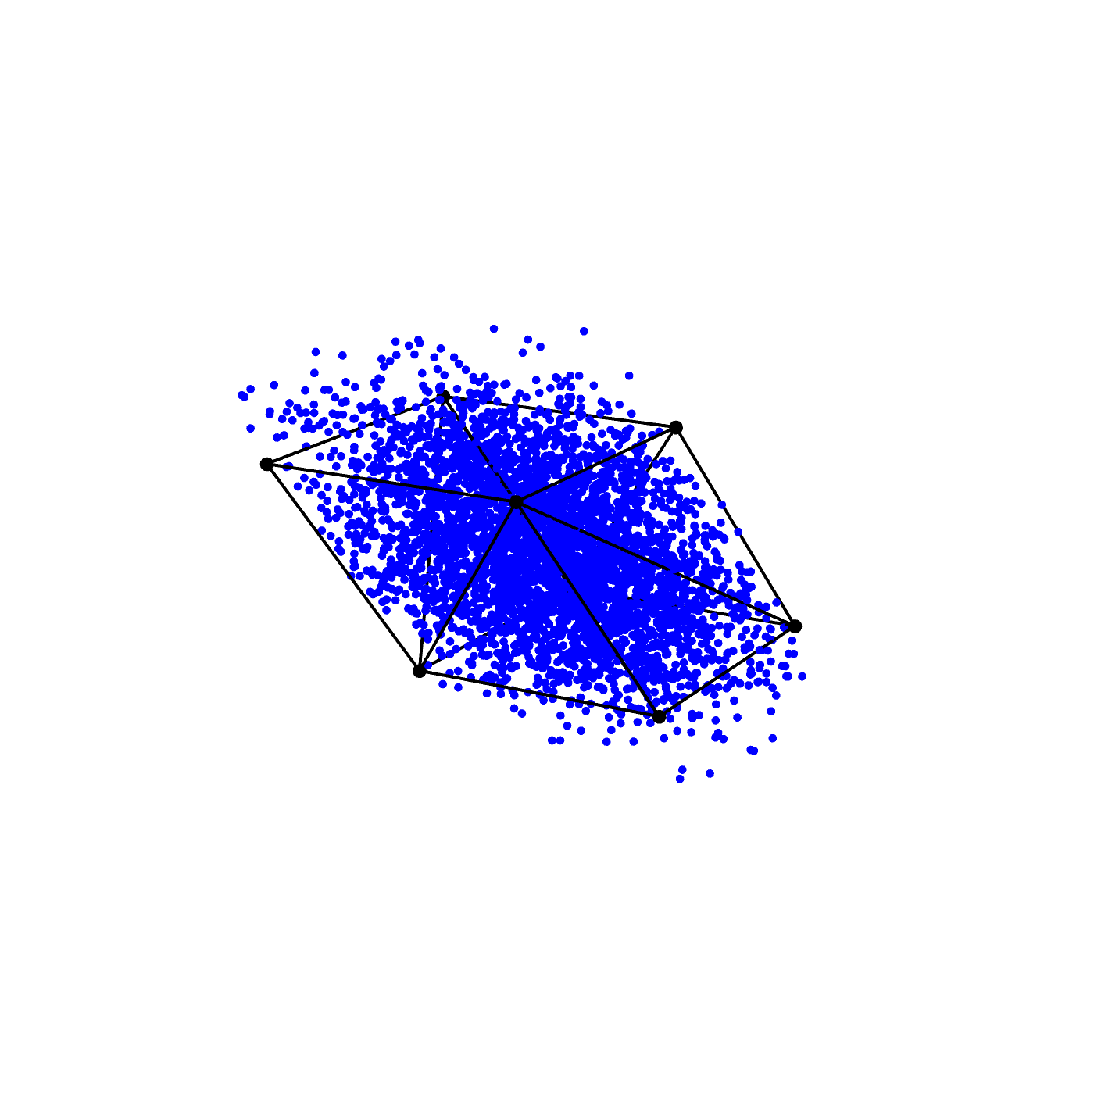
\includegraphics[width=\textwidth]{Abschlussarbeit_2021/LaTeX/images/zonotope_approximation_n3.pdf}
  \end{minipage}\hfill
  \begin{minipage}[b]{0.32\textwidth}
    \centering
    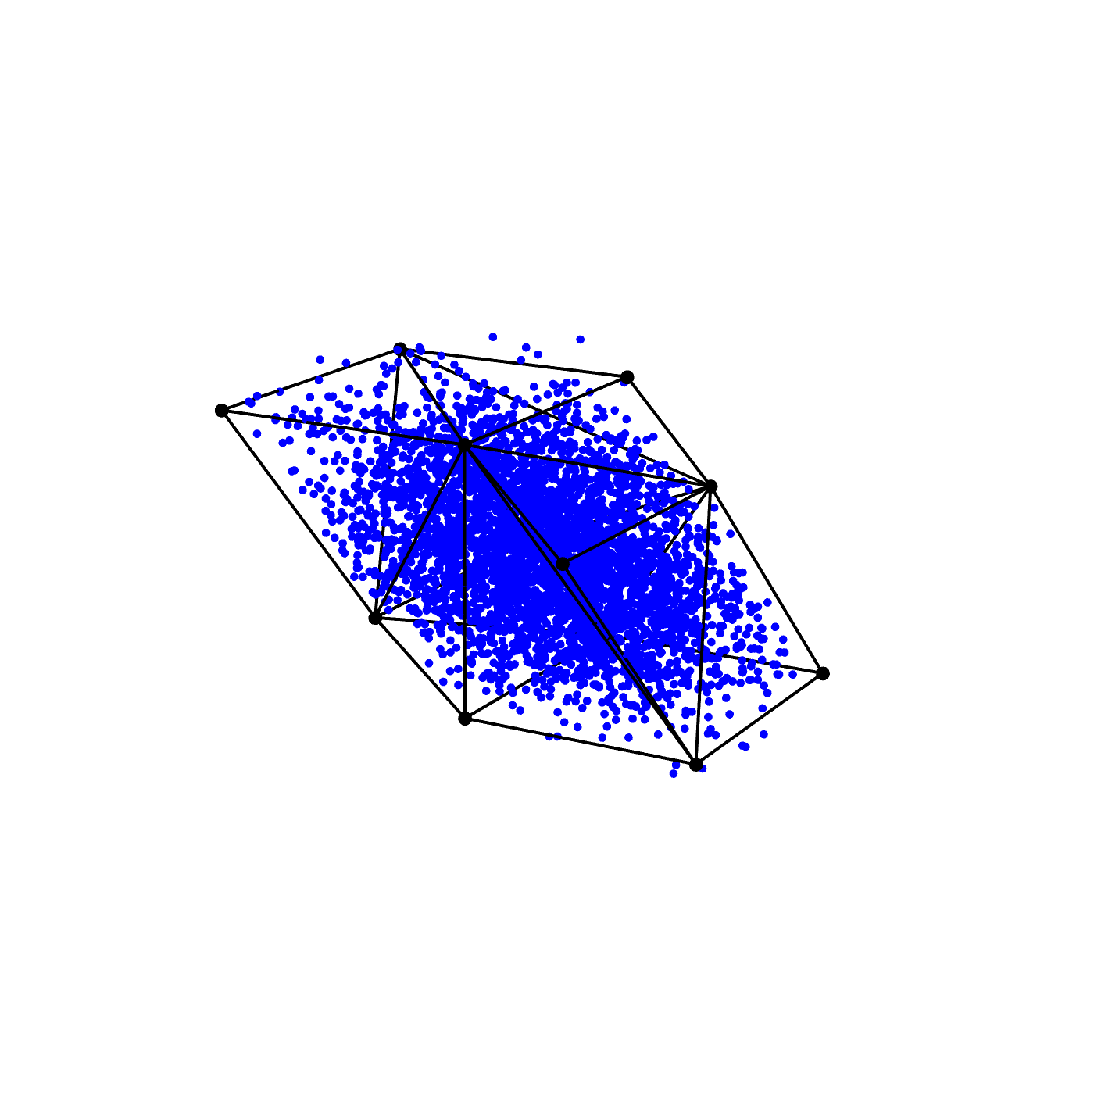
\includegraphics[width=\textwidth]{Abschlussarbeit_2021/LaTeX/images/zonotope_approximation_n4.pdf}
  \end{minipage}\hfill
  \begin{minipage}[b]{0.32\textwidth}
    \centering
    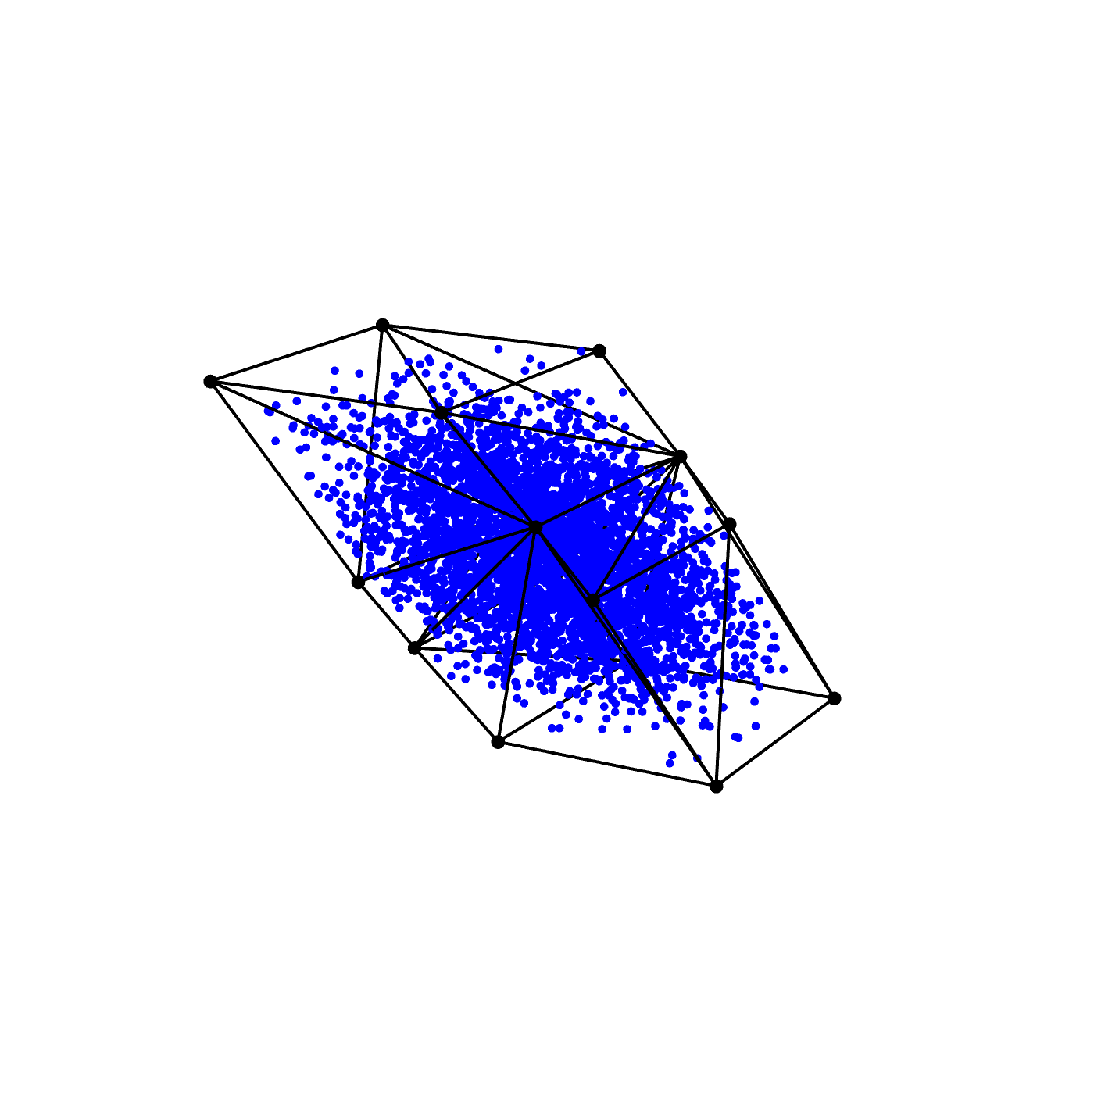
\includegraphics[width=\textwidth]{Abschlussarbeit_2021/LaTeX/images/zonotope_approximation_n5.pdf}
  \end{minipage}

  \caption{Zonotopes approximating the zonoid $\mathcal{Z}$, where $n=3$ (left), $n=4$ (center) and $n=5$ (right)}
  \label{fig:zonotopes}
\end{figure}

\todo[inline]{give approximation quality statement which should connect to the sequence $\psi_j$}

\todo[inline]{Formula for corner points?}

In the case of uniform innovations $Z_t\sim\mathcal{U}[-1,1]$ the points also lie between the hyperplanes with the same form as the central hyperplane, but with affine parts $-1$ and $1$. See Figure~\ref{fig:3d_emb_ar2}.

\begin{figure}[ht]
    \centering
    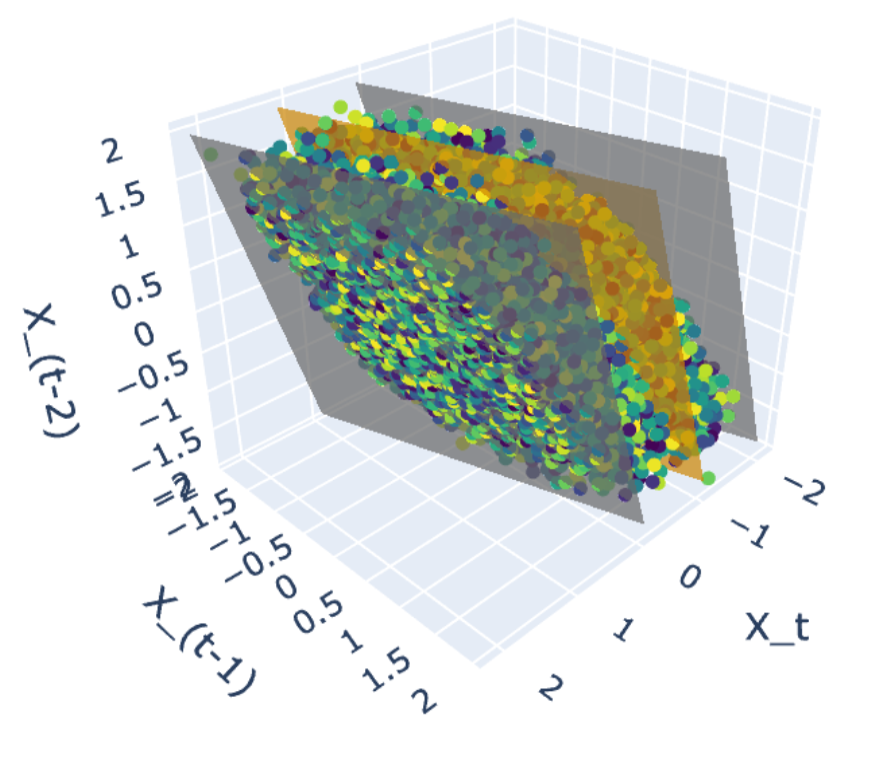
\includegraphics[width=0.5\linewidth]{Abschlussarbeit_2021/LaTeX/images/3d_emb_ar2_cropped.png}
    \caption{Sliding-window embedding ($k=3$) of an AR(2) process. The orange plane is the central plane (right side = 0), the two gray planes are the planes with affine parts -1 and 1 (due to the innovations being $\mathcal{U}[-1,1]$ distributed)}
    \label{fig:3d_emb_ar2}
\end{figure}

If $k>p+1$, the point $Y_t^{(k)}$ lies inside the intersection of multiple slabs:
\begin{align*}
    &\left\{(x_0,\dots,x_{k-1})\in\mathbb{R}^{k}:\begin{array}{l}
    -1\le x_j-\phi_1x_{j+1}-\dots-\phi_px_{j+p}\le 1,\\
    j=0,\dots,k-p-1 
    \end{array}\right\}\\&
    \bigcap_{j=0}^{k-p-1}\left\{(x_0,\dots,x_{k-1})\in\mathbb{R}^{k}:-1\le x_j-\phi_1x_{j+1}-\dots-\phi_px_{j+p}\le 1\right\}
\end{align*}

\todo[inline]{Set $p=1$ and $k=3$, visualize the intersection of slabs}

The distance between the two restricting hyperplanes is given by the formula
\begin{align*}
    d=\frac{2}{\sqrt{1+\phi_1^2+\dots+\phi_p^2}}
\end{align*}

\begin{Def}[Support function]
    Let $K\subseteq\mathbb{R}^{d}$ be a convex nonempty set. The support function of $K$ is $h_K:\mathbb{R}^d\to\mathbb{R}$, $h_K(u)=\sup\{\langle x,u\rangle:x\in K\}$.
\end{Def}

A convex body is a compact nonempty convex set. 

\begin{Lem}
    Let $K,L\subseteq\mathbb{R}^d$ be two convex bodies. Then
    \begin{align*}
        d_H(K,L)=\sup_{u\in S^{d-1}}|h_{K}(u)-h_{L}(u)|.
    \end{align*}
\end{Lem}

The support function of a zonotope is particularly easy: $h_{\mathcal{Z}_n^{(k)}}(u)=\sum_{j=0}^{n}\langle g_j^{(k)},u\rangle$. The width in direction $u$ is given by
\begin{align*}
    w_k(u)=h_{\mathcal{Z}_n^{(k)}}(u)+h_{\mathcal{Z}_n^{(k)}}(-u)=2h_{\mathcal{Z}_n^{(k)}}(u)
\end{align*}
Consider the case $k\ge p+1$. We have
\begin{align*}
    \min_{u\in S^{k-1}}w_k(u)=\frac{2}{\sqrt{1+\phi_1^2+\dots+\phi_p^2}}
\end{align*}
This minimum is attained at the finite set of points
\begin{align*}
    \left\{\pm\frac{q_r^{(k)}}{\|q_{\phi}\|_2}:r=0,\dots,k-(p+1)\right\}
\end{align*}
where $q_{\phi}=(1,-\phi_1,\dots,-\phi_p)$ and
\begin{align*}
    q_r^{(k)}=(\underbrace{0,\dots,0}_{r},1,-\phi_1,\dots,-\phi_p,0,\dots,0)\in\mathbb{R}^{k}
\end{align*}

\todo[inline]{What about $k<p+1$? Is $\min w_k(u)>2^{-1}\sqrt{1+\phi_1^2+\dots+\phi_p^2}$}

An empirical version is given by
\begin{align*}
    \hat{w}_k(u)&=\max_{t}\langle u,Y_t^{(k)}\rangle-\min_{t}\langle u,Y_t^{(k)} \rangle\\
    \hat{m}_k&=\min_{u\in S^{k-1}}\hat{w}_k(u)
\end{align*}

\todo[inline]{Give some convergence result $\hat{w}_k(u)\to w_k(u)$ or $m_k\to\hat{m}_k$}

The idea is to minimize $\hat{w}_k(u)$ over all $u\in S^{k-1}$ and examine the relation $k\mapsto \hat{m}_k$. \textcolor{red}{Unfortunately this minimization problem is very hard.}

\todo[inline]{show numerical results for $p=1,2,3,\dots$}
\todo[inline]{compare $k\mapsto\min w_k(u)$ and $k\mapsto\min\hat{w}_k(u)$}
\todo[inline]{How should the scale similarity matrix be defined?}

For such minimization problems viable methods exist, but the real problem is, that the points $Y_t^{(k)}$ do not fill the support $\mathcal{Z}_k$ well. Rigorously speaking, the convergence of the convex hull of $\mathcal{P}_k$ to $\mathcal{Z}_k$ is of the order $O((\frac{\log n}{n})^{2/(k+1)})$.

\subsection{Normally distributed innovations}

Next, we turn our attention to Gaussian innovations, which is often seen as the default case, that is, $Z_t\sim N(0,\sigma^2)$ for some $\sigma>0$. Using the MA($\infty$) representation, we see that $Y_t^{(k)}\sim\mathcal{N}(0,\Gamma_k)$ with covariance matrix
\begin{align*}
    \Gamma_k=\sigma^2\sum_{j=0}^{\infty}g_j^{(k)}(g_j^{(k)})^{T}
\end{align*}
The covariance matrix plays an important role in describing the geometry of the point cloud $\mathcal{P}_k$. Let $E_c=\{y\in\mathbb{R}^k:y^{T}\Gamma_k^{-1}y\le c\}$ be the ellipsoid of size $c>0$. Then for all $\alpha\in(0,1)$ we have
\begin{align*}
    E_{c_{\alpha}}\in\arg\min\left\{\operatorname{Vol}(A):\mathbb{P}(Y\in A)\ge\alpha:A\subseteq\mathbb{R}^{k}\right\}
\end{align*}
That is, the ellipsoid with size $c_{\alpha}$ is the set with minimum volume, such that the probability that $Y$ is inside $E_{c_{\alpha}}$ is at least $\alpha$.

\todo[inline]{find reference or prove}

\subsection{Heavy-tailed innovations}

\todo[inline]{TBD}

\subsection{Intrinsic Volumes}

\todo[inline]{Handbook of Convex Geometry}

We have a zonotope $Z^{(n)}_k=\sum_{j=0}^{n}g_j[-1,1]$ with \textcolor{red}{unknown} vectors $g_j\in\mathbb{R}^k$. Here, $k$ is the embedding dimension. The $j$-th quermassintegral of $Z^{(n)}_k$, denoted by $W_j(Z^{(n)})$ are defined as coefficients that fulfill
\begin{align*}
    \operatorname{Vol}(Z^{(n)}_k+tB)=\sum_{j=0}^{k}\binom{k}{j}W_j(Z^{(n)}_k)t^{j}
\end{align*}
where $B=B(0,1)=\{x\in\mathbb{R}^k:\|x\|\le1\}$. The $j$-th intrinsic volume is defined by
\begin{align*}
    V_j(Z^{(n)}_k)=\binom{k}{j}\frac{W_{k-j}(Z^{(n)}_k)}{\kappa_{k-j}}, && j=1,\dots,k
\end{align*}
It can be shown that the $j$-th intrinsic volume can by computed by the formula
\begin{align*}
    V_j(Z^{(n)}_k)=2^{j}\sum\limits_{I\subseteq\{0,\dots,n\},|I|=j}\sqrt{\det{(G_I^TG_I)}}
\end{align*}

\subsection{Scale selection for Geometric Approach}

We can fill our scale similarity matrix $\Sigma^{(n)}=\left(\Sigma^{(n)}_{kl}\right)$ with the entries
\begin{align*}
    \Sigma^{(n)}_{kl}=f\left(Z_k^{(n)}\right)+f\left(Z_l^{(k)}\right)-f\left(Z_k^{(n)}\oplus Z_l^{(n)}\right),
\end{align*}
where $\oplus$ is an operation that takes two zonotopes and combines them into a new zonotope. Such an operation can be the following:
\begin{align*}
    Z_k^{(n)}\oplus Z_{l}^{(n)}=\sum_{j=0}^{n}[-1,1]\phi_{k}\left(g_j^{(k)}\right)+
    \sum_{j=0}^{n}[-1,1]\phi_l\left(g_j^{(l)}\right)
\end{align*}
Here, the sum is understood as Minkowski-sum. The Minkowski-sum of two zonotopes is again a zonotope, that is, $Z_k^{(n)}\oplus Z_l^{(n)}$ is again a zonotope. Prior to that we have to apply an embedding $\phi_k:\mathbb{R}^{k}\to\mathbb{R}^{k_{\max}}$, $k=1,\dots,k_{\max}$ with $\phi_k((x_1,\dots,x_k))=(x_1,\dots,x_k,x_{k+1},\dots,x_{k_{\max}})$ (the first $k$ coordinates are preserved).


We can choose $f=V_j$, $j=1,\dots,k$ as functional.

\todo[inline]{Big Question: How to generalize this approach for a wide class of innovation distributions? We only get the nice zonotope formulas because of uniform innovations}

\todo[inline]{Maybe find a class of distributions where the highest density region (or minimum volume set) has a nice geometric shape and compute the intrinsic volumes of that shape}





\section{Numerical Results}

\begin{itemize}
    \item AR($p$) for $p=1,2,3$
    \item different innovations
    \item compare with classical order selection
    \item finite sample stability $(X_1,\dots,X_T)$, $T=200,500,1000$
\end{itemize}






\chapter{Spectral Scale Selection for Kernel Density Estimation}

In this chapter, we apply the scale selection methodology from chapter~\ref{chap:intro_meth} to a sequence of kernel density estimates $\{\hat{f}_{h_i}\}_{i=1}^{N}$.

\section{Preliminaries on Kernel Density Estimation}

We have data $X_1,\dots.X_n\in\mathbb{R}^{d}$ sampled from an (unknown) distribution with density $f$. The kernel density function $\hat{f}_h$ estimates this unknown density. It is defined by
\begin{align*}
    \hat{f}_h(x)\coloneqq \frac{1}{nh^d}\sum_{j=1}^{n}K\left(\frac{x-X_j}{h}\right),\quad x\in\mathbb{R}^d.
\end{align*}

Two common choices for the kernel $K$ are:
\begin{itemize}
    \item the Epanechnikov kernel $K(u)=\mathbf{1}\{-1\le u\le1\}3(1-u^2)/4$
    \item the Gaussian kernel $K(u)=(2\pi)^{-1/2}\exp{(-u^2/2)}$
\end{itemize}

From now on, we always work with the Gaussian kernel, if not indicated otherwise.

The question of how to choose the bandwidth $h$ is widely known in the literature. See reviews~[]. We present some of the most popular methods below, which we also use to compare with our newly developed spectral selector. Following the review~\cite{heidenreich_bandwidth_2013}, bandwidth selectors can be divided into several classes, including plug-in and cross-validation methods. The methods of both classes minimize some approximation of the (mean) integrated squared error.

\begin{Def}
    Let $f$ be a density and $\hat{f}_h$ its kernel density estimate. The integrated squared error (ISE) between $f$ and $\hat{f}_h$ is given by
    \begin{align*}
        \operatorname{ISE}(h)\coloneqq \int\left(f(x)-\hat{f}_h(x)\right)^2\,dx.
    \end{align*}
    The mean integrated squared error (MISE) is $\operatorname{MISE}(h)\coloneqq\mathbb{E}[\operatorname{ISE}(h)]$.
\end{Def}



\subsection*{Cross-variance methods}

The ISE can be written as
\begin{align*}
    \operatorname{ISE}(h)=\int\hat{f}_h(x)^2\,dx-2\mathbb{E}_{X\sim f}\left[\hat{f}_h(X)\right]+\int f(x)^2\,dx
\end{align*}

The Ordinary Least Squares Cross-Variance estimator is given by
\begin{align*}
    \operatorname{CV}(h)=\int\hat{f}_h(x)\,dx-\frac{2}{n}\sum_{i=1}^{n}\hat{f}_{h,-i}(X_i),\quad\hat{h}_{\operatorname{CV}}\in\arg\min\operatorname{CV}(h)
\end{align*}
Here, $\hat{f}_{h,-i}$ is the kernel density function where the observation $X_i$ is left out, that is,
\begin{align*}
    \hat{f}_{h,-i}(x)=\frac{1}{(n-1)h}\sum_{j\ne i}K\left(\frac{x-X_j}{h}\right)
\end{align*}

\subsection*{Plug-in methods}

The bias-variance decomposition of the MISE is
\begin{align*}
    \operatorname{MISE}(h)=\int\operatorname{Var}[\hat{f}_h(x)]\,dx+\int\operatorname{Bias}(\hat{f}_h(x))\,dx
\end{align*}
with
\begin{align*}
    \operatorname{IV}(h)&=\int\operatorname{Var}[\hat{f}_h(x)]\,dx=\frac{\|K\|_2^2}{nh^{d}}-\frac{\|K_h\ast f\|_2^2}{n},\quad\text{and}\\
    \operatorname{ISB}(h)&=\int\operatorname{Bias}(\hat{f}_h(x))\,dx=\|K_h\ast f-f\|_2^2
\end{align*}

This decomposition gives conditions on $h=h_n$ so that the kernel density estimate $\hat{f}_{h_n}$ is consistent. Namely, it must hold $h_n\to0$ and $nh_n^d\to+\infty$. An example of such a sequence is $h_n=cn^{-\alpha}$ for some $c>0$ and $\alpha\in(0,1)$.

The MISE can be written as
\begin{align*}
    \operatorname{MISE}(h)=\underbrace{\frac{\|K\|_2^2}{nh}+\frac{h^4}{4}\mu_2(K)^2\|f^{''}\|_2^2}_{=\operatorname{AMISE}(h)}+o\left(\frac{1}{nh}+h^{4}\right)
\end{align*}

Minimizing the AMISE leads to
\begin{align}\label{eq:h_amise}
    h_{\operatorname{AMISE}}=\left(\frac{\|K\|_2^2}{n\mu_2(K)^2\|f^{''}\|_2^2}\right)^{1/5}
\end{align}

\todo[inline]{check for general dimension $d$}

The optimal bandwidth thus behaves like $n^{-1/5}$.

Plug-in methods use Equation~\eqref{eq:h_amise} as starting point. Silverman's rule of thumb assumes that $f$ is the density of a normal distribution $N(0,\sigma^2)$. In this case, $\|f^{''}\|_2^2$ can simply be computed and plugged into Equation~\eqref{eq:h_amise}:
\begin{align*}
    \|f^{''}\|_2^2=\frac{3}{8\sqrt{\pi}\sigma^{5}},\quad h_{\operatorname{AMISE}}=\left(\frac{4}{3}\right)^{1/5}\sigma n^{-1/5}\approx1.06\sigma n^{-1/5}
\end{align*}

\todo[inline]{introduce (improved) Sheather and Jones' plug in}

\subsection*{Exact MISE representation for Gaussian mixture model}

Exact computations are generally not possible since the true density $f$ of the sampled data $X_1,\dots,X_n$ is not known. In simulation experiments, of course, we simulate the data ourselves and thus know the density $f$. For certain choices of the true density $f$, explicit formulas for the MISE exist.


A particularly broad and well studied class is that of Gaussian mixture models. They are characterized by densities $f$ of the form $f=\sum_{l=1}^{L}w_l\phi_{m_l,\sigma_l^2}$, where $w_l>0$, $\sum_lw_l=1$, $m_l\in\mathbb{R}$, and $\sigma_l^2>0$.

Marron and Wand~\cite{10.1214/aos/1176348653} derive an explicit formula for the MISE between a density $f$ of the Gaussian mixture model and its kernel density estimate with Gaussian kernel of order $r\in\mathbb{N}$. Here we state the formula for the special case $r=1$, that is, for the standard Gaussian kernel.

\begin{Prop}
    The mean integrated squared error between a kernel density estimate $\hat{f}_h$ with Gaussian kernel and the density function $f$ of a Gaussian mixture model with weights $w_l$, variances $s_l^2$ and means $m_l$ is given by
    \begin{align*}
        \operatorname{MISE}(h)&=\frac{1}{2\sqrt{\pi}}\frac{1}{nh}+\left(1-\frac{1}{n}\right)\mathcal{K}(h,2)-2\mathcal{K}(h,1)+\mathcal{K}(h,0),\\
        \mathcal{K}(h,q)&=\sum_{l,l'=1}^{L}\frac{w_lw_{l'}}{\sqrt{s_l^2+s_{l'}^2+qh^2}}\phi\left(\frac{m_l-m_{l'}}{\sqrt{s_l^2+s_{l'}^2+qh^2}}\right),\quad q\in\{0,1,2\}.
    \end{align*}
\end{Prop}



Minimizing $\operatorname{MISE}(h)$ yields the \enquote{oracle} bandwidth $h_{\text{oracle}}$. We will use the oracle bandwidth as an ultimate benchmark in all settings where $\operatorname{MISE}$ has an explicit representation and thus can be minimized using standard methods.


\subsection*{Constructing Mixture Models with multiple global MISE minima}

\todo[inline]{Discuss uniqueness of MISE curve for Gaussian mixture models}



Since the optimal bandwidth minimizes the MISE, particularly interesting scenarios arise in cases where the MISE has no unique minimum. 

Since for Gaussian kernels and Gaussian mixture densities the mean integrated squared error has a closed form, we can find $w_l$, $m_l$, $s_l^2$ such that there exist $h_1<h_2$ that are both global minima of the MISE curve.

\todo[inline]{add construction principle and example, there are different classes of local minima pairs}

This serves as an easy example of a situation where the optimal bandwidth is not unique and thus is a particularly interesting test for spectrally selected bandwidths.

Figure~\ref{fig:equal-minima-example} illustrates a Gaussian mixture density with two local MISE minima.

\begin{figure}[htbp]
    \centering
    \begin{subfigure}{0.48\textwidth}
        \centering
        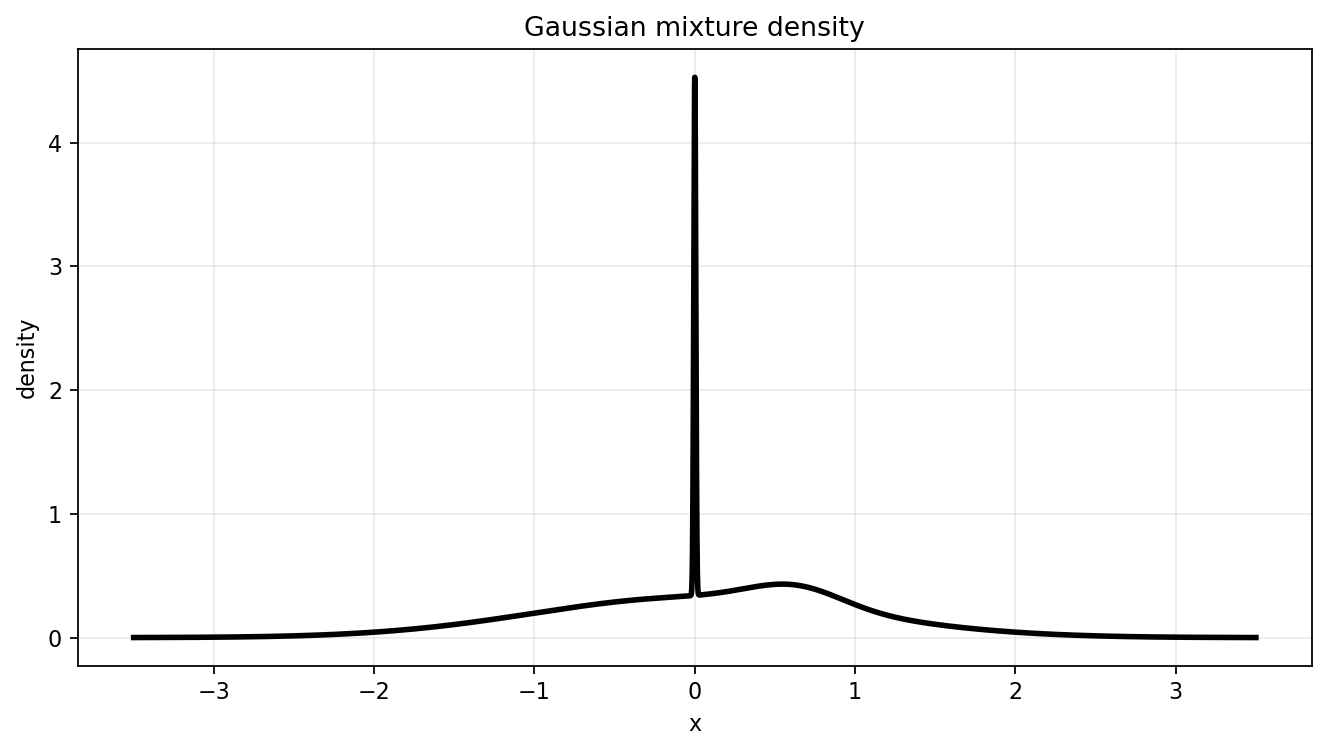
\includegraphics[width=\linewidth]{Code/Code_kde/outputs/equal_minima_mixture_pdf_clean.png}
        \caption{Gaussian mixture density.}
        \label{fig:equal-minima-density}
    \end{subfigure}
    \hfill
    \begin{subfigure}{0.48\textwidth}
        \centering
        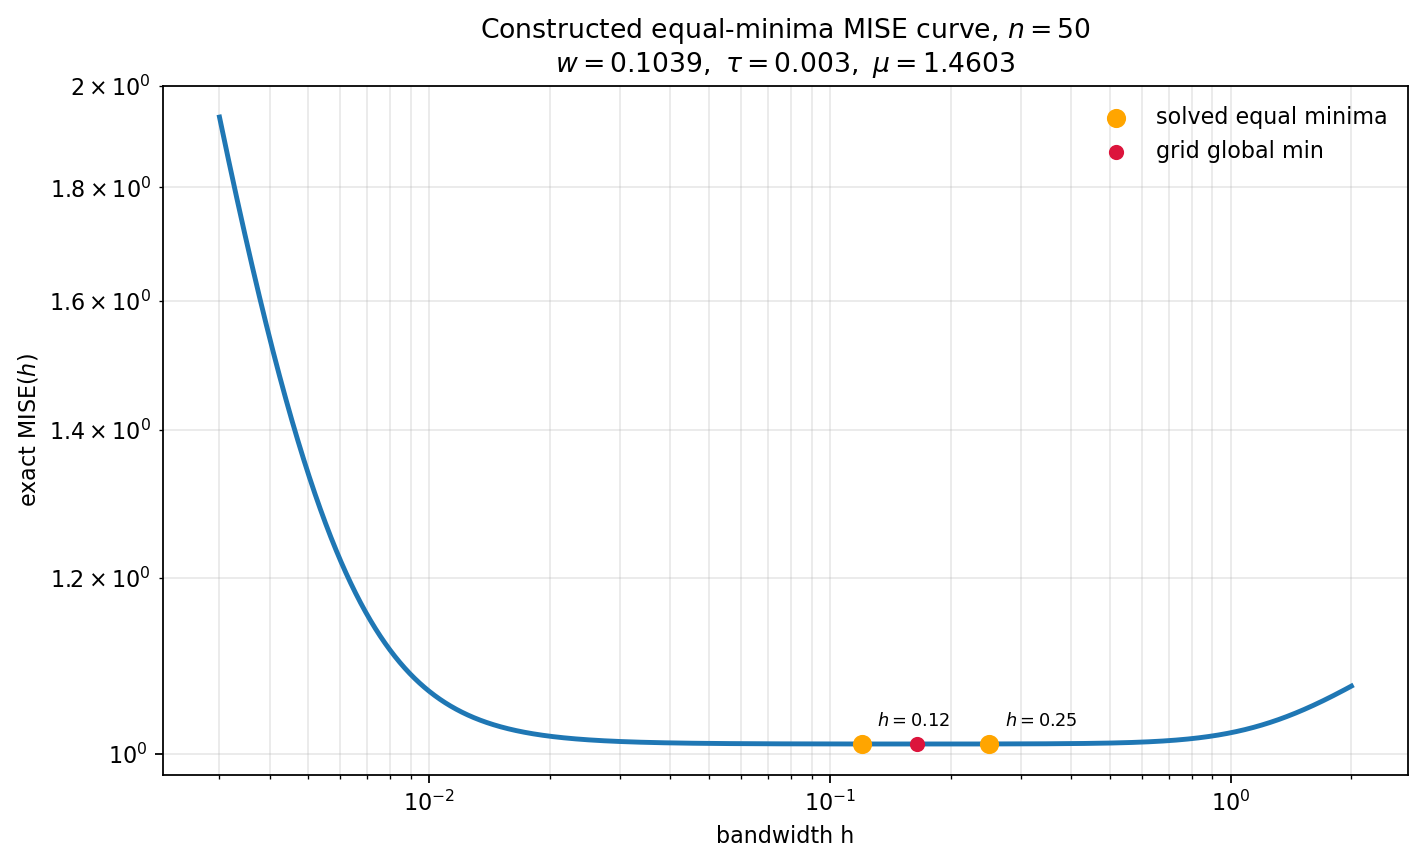
\includegraphics[width=\linewidth]{Code/Code_kde/outputs/mise_equal_minima_constructed.png}
        \caption{Exact MISE curve.}
        \label{fig:equal-minima-mise}
    \end{subfigure}

    \caption{Example of a Gaussian mixture density whose exact MISE curve has two equal local minima.}
    \label{fig:equal-minima-example}
\end{figure}

\section{Divergences between distributions}

\todo[inline]{Introduce the general definition that uses manifolds}

We follow the survey~\cite{nielsen_elementary_2020}.

Let $\mathcal{P}$ be the set of all absolutely continuous probability distributions on $(\mathbb{R}^d,\mathcal{B}(\mathbb{R}^d))$. That is,
\begin{align*}
    \mathcal{P}=\{\mu:\exists f:\mathbb{R}\to\mathbb{R}\text{ measurable},f\ge0,\mu(F)=\int_Ff\,d\lambda\}
\end{align*}

A divergence is a map $D:\mathcal{P}\times\mathcal{P}\to\mathbb{R}_{\ge0}$ such that $D(p,q)=0$ if and only if $p=q$.

The two most important classes of divergences are $f$-divergences and Bregman divergences.

\subsection{\texorpdfstring{$f$}{f}-divergences}

\subsubsection*{Definition and Motivation}

\todo[inline]{Connect $f$-divergence to generalized entropy}

Let $f:\mathbb{R}_{\ge0}\to\mathbb{R}\cup\{+\infty\}$ be a convex function. The $f$-divergence is defined as
\begin{align*}
    D_f(p\|q)=\int f\left(\frac{p(x)}{q(x)}\right)q(x)\,dx
\end{align*}

The $f$-divergence is symmetric iff $f(t)=tf(1/t)+c(t-1)$ for some constant $c$. In particular, the $\alpha$-divergence is symmetric iff $\alpha=1/2$ (Hellinger distance). The only symmetric $\chi^{\alpha}$-divergence is the total variation distance. The JS-divergence is also symmetric.

\todo[inline]{Cite or prove the symmetry characterization}

\subsubsection*{Amari alpha divergence}

A prominent parametrized family of $f$-divergences is the so called $\alpha$-divergence (see \cite{cichocki_families_2010}) where the function $f=f_{\alpha}$ is given by
\begin{align*}
    f_{\alpha}(t)=\frac{1}{\alpha(\alpha-1)}\left(t^{\alpha}-\alpha t-(1-\alpha)\right)
\end{align*}
The actual divergence is then given by
\begin{align*}
    D_{\alpha}(p\|q)=\frac{1}{\alpha(\alpha-1)}\left(\int p(x)^{\alpha}q(x)^{1-\alpha}\,dx-1\right)
\end{align*}

By taking the limit $\alpha\to1$ we recover the Kullback-Leibler divergence, whereas taking the limit $\alpha\to0$ recovers the reverse Kullback-Leibler divergence. At $\alpha=1/2$ we obtain $D_{1/2}(p\|q)=4D_H(p,q)$, where $D_H(p,q)=(1/2)\int(\sqrt{f}-\sqrt{g})^2$ is the squared Hellinger distance.

\todo[inline]{Mention two different parameterizations}

\subsubsection*{chi squared divergence (total variance)}

Another class of divergences are the $\chi^{\alpha}$-divergences (see~[]). They are determined by $f_{\alpha}(t)=(1/2)|t-1|^{\alpha}$, where $\alpha\ge1$. Setting $\alpha=1$ recovers the well known total variation distance: $d_{\text{TV}}(p,q)=(1/2)\int|p-q|$.

\subsubsection*{JS divergence}

Another important divergence that belongs to the class of $f$-divergences is the Jensen Shannon divergence. The function $f$ is set to be
\begin{align*}
    f(t)=\frac{1}{2}\left(t\log{t}-(t+1)\log{\frac{t+1}{2}}\right)
\end{align*}
The divergence is then given by
\begin{align*}
    \operatorname{JS}(f,g)=H\left(\frac{f+g}{2}\right)-\frac{1}{2}H(f)-\frac{1}{2}H(g),
\end{align*}
where $H(f)=-\int f\log{f}$ is the Shannon entropy.

\subsubsection*{Renyi divergence}

The class of Rényi divergences is defined as
\begin{align*}
    R_{\alpha}(p\|q)=\frac{1}{\alpha-1}\log{\left(\int p(x)^{\alpha}q(x)^{1-\alpha}\,dx\right)},
\end{align*}
where $\alpha\in\mathbb{R}\setminus\{1\}$ is the order. In case of $\alpha>1$, we read $f^{\alpha}g^{1-\alpha}=f^{\alpha}/g^{\alpha-1}$. The limiting case $\alpha\to1$ recovers the Kullback-Leibler divergence.

The Rény divergence and the $\alpha$-divergence are different transformations of the same integral $C_{\alpha}(p,q)=\int p^{\alpha}q^{1-\alpha}$. We have
\begin{align*}
    R_{\alpha}(p\|q)&=g(C_{\alpha}(p,q)),\quad g(t)=\frac{1}{\alpha-1}\log{t}\\
    D_{\alpha}(p\|q)&=h(C_{\alpha}(p,q)),\quad h(t)=\frac{1}{\alpha(\alpha-1)}(t-1)
\end{align*}

\todo[inline]{transformations in each other}

By Hölders inequality $0\le C_{\alpha}(p,q)\le 1$.

\subsection{Bregman divergences}

The second major class are Bregman divergences, which are defined by
\begin{align*}
    D_F(p\| q)=F(p)-F(q)-\langle\nabla F(q),p-q\rangle,
\end{align*}
where $F\in C^{1}$. A particular subclass is given by
\begin{align*}
    F_{\phi}(p)=\int\phi(p(x))\,dx
\end{align*}
for some convex function $\phi$. An example of such a function $\phi$ is the class of $\beta$-divergences determined by
\begin{align*}
    \phi_{\beta}(t)=\frac{t^{1+\beta}}{\beta(\beta+1)},\quad\beta\in\mathbb{R}\setminus\{0,-1\}
\end{align*}

\todo[inline]{Condition on $F$ or $\phi$ under which Bregman divergence is symmetric}

The $\beta$-divergence is thus given by
\begin{align*}
    D_{\beta}(p,q)=\frac{1}{\beta(\beta-1)}\left(\int p^{\beta}+(\beta-1)\int q^{\beta}-\beta\int pq^{\beta-1}\right)
\end{align*}

For $\beta=2$ we get
\begin{align*}
    D_2(p,q)=\frac{1}{2}\int(p-q)^2=\frac{1}{2}\|p-q\|_2^2
\end{align*}

If $p(x)=\hat{f}_h(x)=n^{-1}\sum_jK_h(x-X_j)$ and $q(x)=\hat{f}_s(x)=n^{-1}\sum_jK_h(x-X_j)$ are kernel density estimates with a Gaussian kernel $K$, we can obtain an explicit formula for $D_2(\hat{f}_h,\hat{f}_s)$. We have
\begin{align}\label{eq:exact_l2_divergence}
    D_2(\hat{f}_h,\hat{f}_s)=\frac{1}{2n^2}\sum_{i,j}\left(\phi_{\sqrt{2}h}(X_i-X_j)+\phi_{\sqrt{2}s}(X_i-X_j)-\phi_{\sqrt{h^2+s^2}}(X_i-X_j)\right)
\end{align}
The derivation of the formula uses mainly the Gaussian convolution identity, that is, the fact that for Gaussian densities $f_1=\phi_{\mu_1,\sigma_1^2}$ and $f_2=\phi_{\mu_2,\sigma_2^2}$ their convolution is $f_1\ast f_2=\phi_{\mu_1+\mu_2,\sigma_1^2+\sigma_2^2}$.

\subsubsection*{Relations between all presented divergences}

\todo[inline]{Do all these divergences relate to each other?}

\begin{Prop}
    Let $D$ be a divergence such that it is a $f$-divergence for some $f$ and simultaneously a Bregman divergence for some $F$. This is sufficient and necessary for $D$ to be the Kullback-Leibler divergence.
\end{Prop}

\section{Assembly of Scale Similarity Matrices}

A matrix $A\in\mathbb{R}^{n\times n}$ is positive definite if $x^TAx>0$ for all $x\in\mathbb{R}^n$, $x\ne0$. A symmetric map $D:X\times X\to\mathbb{R}$ with $D(x,x)=0$ is called conditionally negative definite if
\begin{align*}
    \sum_{i,j=1}^{n}a_ia_jD(x_i,x_j)\le0
\end{align*}
for all $x_1,\dots,x_n\in X$ and $a_1,\dots,a_n\in\mathbb{R}$ with $\sum_{i}a_i=0$. A function $\phi:(0.\infty)\to\mathbb{R}$ is called completely monotone if $\phi\in C^{\infty}(0,\infty)$ and $(-1)^{n}\phi^{(n)}(t)\ge 0$ for all $n\in\mathbb{N}_0$ and $t>0$.

\todo[inline]{Which divergencies are conditionally negative definite and which not; Jensen Shannon? (Fuglede and Topsøe)}

The most prominent example of a completely monotone function is $\phi(t)=e^{-\gamma t^{\alpha}}$, $\gamma\ge0$, $0<\alpha\le1$.

\begin{Thm}[Schoenberg]\label{thm:schoenberg}
    Let $D:X\times X\to\mathbb{R}$ be conditionally negative. Let $x_1,\dots,x_n\in X$. If $\phi$ is completely monotone, then the matrix $\Sigma=(\Sigma_{ij})$, $\Sigma_{ij}=\phi(D(x_i,x_j))$ is positive definite.
    \todo[inline]{Find a source to cite}
\end{Thm}

\todo[inline]{connect to Bernstein–Widder}

Theorem~\ref{thm:schoenberg} gives a general construction principle for the scale similarity matrix $\Sigma^{(N)}=(\Sigma^{(N)}_{ij})$. Namely, we set $\Sigma^{(N)}_{ij}=\phi(D(\hat{f}_{h_i},\hat{f}_{h_j}))$ where $D$ is some divergence and $\phi$ a completely monotone function. 

There are some special kinds of divergences, where a transformation by a not necessarily completely monotone function is enough to obtain a positive definite similarity matrix.

\todo[inline]{What is it about these special divergences that do not require a completely monotone transformation?}

The transformation $S_{ij}=\exp{\{-D_{ij}/\tau\}}$ can be motivated as follows. Let $H(p)=-\sum_jp_j\log{p_j}$ be the entropy of the probability vector $p\in\mathbb{R}^{N}$. The quantity
\begin{align*}
    \sum_{j=1}^{N}p_jD_{ij}-\tau H(p)
\end{align*}
is minimized by $p_i=(p_{i1},\dots,p_{iN})$, where $p_{ij}=S_{ij}/\sum_{k=1}^{N}S_{ik}$. In that sense, $\tau$ can be interpreted as a penalty weight. This is another instance of the Donsker–Varadhan variational principle. See~\cite{anantharam_variational_2017} for reference.

Apply the transformation $\exp{(-\tau D_{\alpha})}$ to the Renyi divergence $D_{\alpha}$ yields
\begin{align*}
    S_{ij}&=\exp{(-\tau D_{\alpha}(\hat{f}_{h_i},\hat{f}_{h_j}))}\\
    &=\exp{\left\{\frac{\tau}{1-\alpha}\log{C_{\alpha}(\hat{f}_{h_i},\hat{f}_{h_j})}\right\}}\\
    &=C_{\alpha}(\hat{f}_{h_i},\hat{f}_{h_j})^{\frac{\tau}{1-\alpha}}
\end{align*}

\subsection*{Why not use the divergence matrix for spectral scale selection?}

In this subsection, we want to briefly give an argument why it is not advisable to compute the Perron vector of the divergence matrix $D$ itself and thus motivate the above similarity transformation more.

\begin{Def}[Robinson matrix]
    A matrix $D$ with entries $D_{ij}=D(x_i,x_j)$ is called a Robinson matrix (cf.~\cite{carmona_two_2024}) if there exists a permutation $\pi$ on $\{1,\dots,N\}$ such that for $D_{ij}^{\pi}=D(x_{\pi(i)},x_{\pi(j)})$ it holds
    \begin{align*}
        D^{\pi}_{ik}\ge\max\{D^{\pi}_{ij},D^{\pi}_{jk}\}\text{ and }D_{ki}^{\pi}\ge\max\{D_{ji}^{\pi},D_{kj}^{\pi}\}
    \end{align*}
    whenever $i<j<k$.
\end{Def}

\todo[inline]{Prove that for Gaussian kernels we obtain a Robinson matrix?}

The reason why we do not want to work with the matrix $D$ and instead transform to a similarity matrix $\phi(D)$ is due to the following Lemma.

\begin{Lem}
    Let $(M,d)$ be a geodesic metric space such that for every fixed point $y\in X$, the function $x\mapsto d(x,y)$ is geodesically convex. Let $X\subseteq M$ be a convex subset. Let $x_1,\dots,x_N\in X$ be finitely many points and define the distance matrix $D=(d(x_i,x_j))_{i,j=1}^{N}$. Let $v=(v_j)\in\mathbb{R}^{N}$ be the Perron vector of $D$. Then
    \begin{align*}
        \arg\max_{1\le j\le N}v_j\subseteq\{1,N\}.
    \end{align*}
    \todo[inline]{Find correct assumptions to prove the Lemma}
    \todo[inline]{This Lemma is not correct yet but numerical experiments suggest that the Perron vector of divergence matrices behaves not how we want}
\end{Lem}

\begin{proof}
    Define the function
    \begin{align*}
        F(x)=\sum_{j=1}^{N}d(x,x_j)v_j,\quad x\in X.
    \end{align*}
    Since $v$ is the Perron vector, we have $F(x_i)=\lambda v_i$. Thus
    \begin{align*}
        \arg\max_{1\le j\le N} v_j=\arg\max_{1\le j\le N}F(x_j).
    \end{align*}
\end{proof}

\subsection*{Approximating integrals using quadrature}

Computing divergences between densities amounts to evaluating integrals of the form $\int_{-\infty}^{+\infty}C_{\alpha}(p,q)$, where, for example, in the case of the $\alpha$ or Rényi divergence, $C_{\alpha}(p,q)=p^{\alpha}q^{1-\alpha}$. In general, these integrals cannot be computed explicitly, and numerical procedures have to be applied. Before that, the integral has to be truncated. The truncation error can be bounded above:
\begin{align*}
    E_{\text{trunc}}=\int\limits_{\mathbb{R}\setminus(a,b)}C_{\alpha}(p,q)\le\left(\int\limits_{\mathbb{R}\setminus(a,b)}p\right)^{\alpha}\left(\int\limits_{\mathbb{R}\setminus(a,b)}q\right)^{1-\alpha}
\end{align*}

We also have
\begin{align*}
    \int\limits_{\mathbb{R}\setminus(a,b)}\hat{f}_{h}=\frac{1}{n}\sum_{j=1}^{n}\underbrace{\int\limits_{\mathbb{R}\setminus(a,b)}\frac{1}{h}K\left(\frac{x-X_j}{h}\right)\,dx}_{=\Phi((a-X_j)/h)+\Phi((X_j-b)/h)}
\end{align*}

Setting $a=X_{\min}-L h_{\max}$ and $b=X_{\max}+Lh_{\max}$, where $X_{\min}=\min X_j$, $X_{\max}=\max X_j$ and $h_{\max}=\max h_i$, we obtain
\begin{align*}
    \Phi((a-X_j)/h)+\Phi((X_j-b)/h)\le2\Phi(-L)
\end{align*}
and thus $E_{\text{trunc}}\le 2\Phi(-L)$. Using the upper bound for the above truncation error, we choose $L$ such that $E_{\text{trunc}}\le\epsilon$. This can be achieved by setting $L\ge\Phi^{-1}(1-\epsilon/2)$.

Afterwards, we use the composite trapezoidal rule to approximate the truncated integral:
\begin{align*}
    \int_a^bf(x)\,dx\approx Q_n(f)=\frac{b-a}{2n}\left(f(a)+2\sum_{k=1}^{n-1}f(x_k)+f(b)\right),
\end{align*}
where $x_k=a+\frac{b-a}{n}k$, $k=0,1,\dots,n$ are the equidistant nodes.

\todo[inline]{cite source for the approximation guaranty}

As an approximation guaranty, we have
\begin{align}\label{eq:approx_error}
    \left|\int_a^bf(x)\,dx-Q_n(f)\right|\le\frac{(b-a)^3}{12}\|f^{''}\|_{\infty}n^{-2}
\end{align}

Adaptive quadrature rules might give better approximation results but are computationally more expensive.

In our application, $f(x)=C_{\alpha}(p(x),q(x))=p(x)^{\alpha}q(x)^{1-\alpha}$. The approximation guaranty of Equation~\eqref{eq:approx_error} then becomes
\begin{align*}
    \left|\int\limits_{X_{\min}-Lh_{\max}}^{X_{\max}+Lh_{\max}}C_{\alpha}(\hat{f}_{h_i},\hat{f}_{h_j})-Q_n(C_{\alpha}(\hat{f}_{h_i},\hat{f}_{h_j}))\right|\le\frac{(X_{\max}-X_{\min}+2Lh_{\max})^3}{12n^2}M_{2,i,j}(\alpha),
\end{align*}
where
\begin{align*}
    M_{2,i,j}(\alpha)
    &=\frac{1}{\sqrt{2\pi}h_i^{\alpha}h_j^{1-\alpha}}
    \Bigg[
    (X_{\max}-X_{\min}+Lh_{\max})^2
    \left(\frac{\alpha}{h_i^2}+\frac{1-\alpha}{h_j^2}\right)^2\\
    &\qquad
    +\alpha\left(
    \frac{1}{h_i^2}
    +\frac{(X_{\max}-X_{\min})^2}{4h_i^4}
    \right)\\
    &\qquad
    +(1-\alpha)\left(
    \frac{1}{h_j^2}
    +\frac{(X_{\max}-X_{\min})^2}{4h_j^4}
    \right)
    \Bigg].
\end{align*}

\todo[inline]{Explain how error depends on $\alpha$, $X_{\max}-X_{\min}$ and the bandwidths $h_i$}

\subsection*{Fast Fourier Transform}

The computation of the divergence matrix $D$ using the exact formula in Equation~\eqref{eq:exact_l2_divergence} is of the order $\mathcal{O}(N^2n^2)$, where $N$ is the size of the bandwidth grid and $n$ the sample size. In order to speed up the computation of $D_{ij}=D(\hat{f}_{h_i},\hat{f}_{h_j})$, we make use of the Fast Fourier Transform (FFT). In the following we will briefly describe the approach by following the book~\cite{plonka_numerical_2018}.

For any function $f\in L_1(\mathbb{R})$ the Fourier transform is defined as $\mathcal{F}:f\mapsto\mathcal{F}[f]$ where $\mathcal{F}[f](\omega)=\int f(x)\exp{(-ix\omega)}\,dx$. The Fourier transform of the Gaussian density $\phi_{\sigma}$ is famously given by $\mathcal{F}[\phi_{\sigma}](\omega)=\exp{(-\sigma^2\omega^2/2)}$. Using the linearity and translation property of the Fourier transform we obtain the Fourier transform of a kernel density function with Gaussian kernel:
\begin{align*}
    \mathcal{F}[\hat{f}_h](\omega)=\underbrace{\left(\frac{1}{n}\sum_{j=1}^{n}\exp{(-iX_j\omega)}\right)}_{=P_n(\omega)}\exp{(-h^2\omega^2)/2}
\end{align*}
Next we use Parseval's identity to get
\begin{align*}
    G_{r,s}=\int\hat{f}_{h_r}(x)\hat{f}_{h_s}(x)\,dx&=\frac{1}{2\pi}\int\mathcal{F}[\hat{f}_h](\omega)\overline{\mathcal{F}[\hat{f}_s](\omega)}\,d\omega\\&
    =\frac{1}{2\pi}\int|P_n(\omega)|^2\exp{(-(h^2+s^2)\omega^2/2)}\,d\omega\\&
    =\frac{1}{\pi}\int_0^{\infty}|P_n(\omega)|^2\exp{(-(h^2+s^2)\omega^2/2)}\,d\omega
\end{align*}

Truncate and apply composite trapezoidal rule
\begin{align*}
    \frac{1}{2\pi}\frac{\Omega}{K}\sum_{k=0}^{K}c_k|P_n(\omega_k)|^2\exp{(-(h_r^2+h_s^2)\omega_k^2/2)}
\end{align*}

The error is bounded above by
\begin{align*}
    \underbrace{\frac{1}{2\sqrt{\pi}h_{\min}}\operatorname{erfc}(h_{\min}\Omega)}_{\text{truncation error}}+\underbrace{\frac{M\Omega^3}{12\pi K^2}}_{\text{quadrature error}},
\end{align*}
where $M=(X_{\max}-X_{\min})^2+2(X_{\max}-X_{\min})h_{\max}\sqrt{2/e}+2h_{\max}^2$. Choose
\begin{align*}
    \Omega&\ge\frac{1}{h_{\min}}\operatorname{erfc}^{-1}(2\sqrt{\pi}h_{\min}\epsilon_{\text{trunc}})\\
    K&\ge\sqrt{\frac{M\Omega^3}{12\pi\epsilon_{\text{quadr}}}}
\end{align*}

\subsection*{Bandwidth grid}

\todo[inline]{Argue why linear grid won't work}

\todo[inline]{grid must scale with $n$? Explain why}

The choice of the correct bandwidth grid is essential. Let $\mathcal{H}=\{h_1,\dots,h_N\}$ with $0<h_{\min}=h_1<\dots<h_N=h_{\max}$. We can choose between a linear or geometric grid, that is,
\begin{align*}
    h_j=h_{\min}+\frac{j-1}{N-1}(h_{\max}-h_{\min})=h_{\min}+q_N(j-1),\quad q_N=\frac{h_{\max}-h_{\min}}{N-1}
\end{align*}
or
\begin{align*}
    h_j=h_{\min}\left(\frac{h_{\min}}{h_{\max}}\right)^{\frac{j-1}{N-1}}=h_{\min}q_N^{j-1},\quad q_N=\left(\frac{h_{\min}}{h_{\max}}\right)^{1/(N-1)}
\end{align*}

\todo[inline]{illustrative image comparing linear and geometric grid with ticks on an interval}

\subsection*{Further considerations}

\todo[inline]{Invent construction that removes the influence on the position in the grid}

We want to eliminate the centrality of each scale $i$ coming purely from its location on the grid. To this end we use the so called Toeplitz projection:
\begin{align*}
    S^{(0)}=(S^{(0)})_{ij},\quad S^{(0)}_{ij}=\overline{S}_{|i-j|},\quad\overline{S}_d=\frac{1}{N-d}\sum_{i=1}^{N-d}S_{i,i+d}
\end{align*}
The Toeplitz projection $S^{(0)}$ of a matrix $S$ is a Toeplitz matrix where the entries of each diagonal is the mean of the corresponding diagonal of $S$. In fact, $S^{(0)}$ is closest to $S$ out of all Toeplitz matrices in terms of the Frobenius norm. See~\cite{kucerovsky_properties_2016}.


Let $v^{(0)}$ be the Perron vector of $S^{(0)}$. Then $v^{(0)}_i$ is a centrality measure of the scale $i$ coming purely from the position in the grid. We define $s_i=v_i/v^{(0)}_i$ which is the null corrected scale centrality. Writing $\log{s_i}=\log{v_i}-\log{v^{(0)}_i}$, we can interpret $\log{v^{(0)}_i}$ as spectral grid penalty. This idea is closely analogous to normalization against a null model.

The fact that the similarity matrix $S$ is not symmetric in general is not a problem because the Doob h transform also works in this case. The resulting stationary distribution $\pi$ is given by
\begin{align*}
    \pi_i=\frac{l_ir_i}{\sum_{j=1}^{N}l_jr_j}
\end{align*}
where $r$ and $l$ are the right and left principal eigenvectors of $S$, that is, $Sr=\lambda_{\max}r$ and $S^{T}l=\lambda_{\max}l$.

\textbf{working hypothesis.} Let $h^*_D=\arg\min\mathbb{E}[D(f,\hat{f}_h)]$ and let $S=\exp{(-D/\tau)}$. Does the peak of the Perron vector of $S$ relate to $h^*_D$?

\section{Numerical Experiments}

Let $X_1,\dots,X_n\sim f$. In our experiments, we focus primarily on the case $f\sim N(0,\sigma^2)$.

Figure~[] shows the relation $i\mapsto\pi_i$, where $\pi$ is the stationary distribution.


Figure~[] shows the stability with respect to the grid fineness $N$. The samples $X_1,\dots,X_n$ were kept fixed.


Figure~[] shows the results of studying the distribution of the chosen bandwidths under repeatedly drawn samples $(X_1^{(i)},\dots,X_n^{(i)})$, $i=1,\dots,M$.


It is interesting to ask what happens to this distribution for increased sample size $n$. The answer is depicted in Figure~[]. The spectrally chosen bandwidths concentrate towards a deterministic interior scale $h^*$.

\chapter{Conclusion}

In the first part of this thesis we developed a new method for estimating the coefficients and determining the order of auto-regressive processes. It is based on the minimization of the width of the sliding window embedding of the AR process via projected sub-gradient descent. By establishing a connection to convex geometry, we were able to derive consistency results for this new method.

The second part of this thesis was concerned about applying the spectral scale selection methodology developed in the manuscript~\cite{Baralic2026} to bandwidth selection in kernel density estimation. We developed a framework for how to construct pairwise similarity matrices using the notion of divergences between probability distributions. Our main result establishes an interesting connection between energy functional minimization and spectral scale selection. 
\chapter{Outlook}

\textbf{Geometric Estimation of Autoregressive processes}

\todo[inline]{Big Question: How to generalize this approach for a wide class of innovation distributions? We only get the nice zonotope formulas because of uniform innovations}

A vital question is how to generalize the approach developed above to a broader class of innovation distributions. The main difficulty to overcome is that $\operatorname{supp}(Y_t^{(k)})$ is generally not compact but usually unbounded. Thus, the minimum width is infinite.

\todo[inline]{Probability integral transform (PIT)}

\todo[inline]{linear filter, Wold representation}

The \textit{minimum volume set} (compare~\cite{JMLR:v7:scott06a}) is defined by
\begin{align*}
    E_{\alpha}\in\arg\min\{\lambda_d(A):\mathbb{P}(Y\in A)\ge\alpha,A\in\mathcal{B}(\mathbb{R}^d)\}.
\end{align*}
The \textit{highest density region} $C_{\alpha}$, $\alpha\in(0,1)$ (see~\cite{Hyndman01051996}) is defined by
\begin{align*}
    C_{\alpha}&=C_{h_{\alpha}}\\
    C_h&=\{x\in\mathbb{R}^{d}:f(x)\ge h\}\\
    h_{\alpha}&=\sup\{h\in\mathbb{R}:\mathbb{P}(Y\in C_h)\ge 1-\alpha\}
\end{align*}

\todo[inline]{connect these concepts with each other. For many distributions they are the same. Using minimum volume sets would remove dependence on having a smooth density}

\todo[inline]{estimate HDR directly from the points $Y_t^{(k)}$; non parametric estimation, empirical HDR}

\todo[inline]{Maybe find a class of distributions where the highest density region (or minimum volume set) has a nice geometric shape and compute the intrinsic volumes of that shape}

\todo[inline]{log concave distributed innovations give convex highest density regions; VERY INTERESTING}

A probability density is log concave if
\begin{align*}
    f(x)=\frac{e^{-V(x)}}{\int e^{-V(u)}\,du}
\end{align*}
for some convex function $V$.

\textbf{Normally distributed innovations}

Next, we turn our attention to Gaussian innovations, which is often seen as the default case, that is, $Z_t\sim N(0,\sigma^2)$ for some $\sigma>0$. Using the MA($\infty$) representation, we see that $Y_t^{(k)}\sim\mathcal{N}(0,\Gamma_k)$ with covariance matrix
\begin{align*}
    \Gamma_k=\sigma^2\sum_{j=0}^{\infty}g_j^{(k)}(g_j^{(k)})^{T}
\end{align*}
The covariance matrix plays an important role in describing the geometry of the point cloud $\mathcal{P}_k$. Let $E_c=\{y\in\mathbb{R}^k:y^{T}\Gamma_k^{-1}y\le c\}$ be the ellipsoid of size $c>0$. Then for all $\alpha\in(0,1)$ we have
\begin{align*}
    E_{c_{\alpha}}\in\arg\min\left\{\operatorname{Vol}(A):\mathbb{P}(Y\in A)\ge\alpha:A\subseteq\mathbb{R}^{k}\right\}
\end{align*}
That is, the ellipsoid with size $c_{\alpha}$ is the set with minimum volume, such that the probability that $Y$ is inside $E_{c_{\alpha}}$ is at least $\alpha$.

\todo[inline]{find reference or prove}

\textbf{Spectral Scale Selection for Kernel Density Estimation}
\chapter{Appendix}\label{chap:appendix}

\section{Proofs Chapter~\ref{chap:ar}}

\subsection{Proof of Proposition~\ref{prop:hausdorff_distance_convergence_speed}}\label{sec:proof_hausdorff_distance_convergence_speed}

\begin{Lem}\label{lem:upper_bound_psi_j}
    There exist $C>0$ and $\rho\in(0,1)$ such that $|\psi_j|\le C\rho^{j}$. In particular, $\lim\limits_{j\to\infty}\psi_j=0$.
\end{Lem}

\begin{proof}
    Define $r_{\phi}:=\min\{|z|:z\in\mathbb{C},\phi(z)=0\}$. Since $\{X_t\}$ is causal, $r_{\phi}>1$. Let $R\in(1,r_{\phi})$ be arbitrary. From complex analysis, it follows that $1/\phi$ is analytical on the disk $D_0(R)=\{z\in\mathbb{C}:|z|\le R\}$. Let $1/\phi(z)=\sum_{j=0}^{\infty}\psi_jz^{j}$ be its representation. By Cauchy's integral inequality, see~\cite[Corollary~4.3]{Shiu01072004}, $|\psi_j|\le R^{-j}\max_{|z|=R}|1/\phi(z)|$. Setting $C=\max_{|z|=R}|1/\phi(z)|$ and $\rho=R^{-1}$ yields the statement.
\end{proof}

\begin{proof}
    First, notice that $\mathcal{Z}_n^{(k)}\subseteq\mathcal{Z}$ for all $n\in\mathbb{N}$ and therefore $d(y,\mathcal{Z}^{(k)})=0$ for all $y\in\mathcal{Z}_n^{(k)}$. By definition of the Hausdorff distance $d_H(\mathcal{Z}_n^{(k)},\mathcal{Z})=\sup\{d(\mathcal{Z}_n^{(k)},z):z\in\mathcal{Z}^{(k)}\}$. Let $y\in\mathcal{Z}_n^{(k)}$ and $z\in\mathcal{Z}^{(k)}$ be arbitrary. They have representations $\sum_{j=0}^{n}a_jg_j^{(k)}$ and $\sum_{j=0}^{\infty}b_jg_j^{(k)}$ respectively for some $a_j,b_j\in[-1,1]$. Now we have
    \begin{align*}
        d(y,z)&=\left\|\sum_{j=0}^{n}a_jg_j^{(k)}-\sum_{j=0}^{\infty}b_jg_j^{(k)}\right\|=\left\|\sum_{j=n+1}^{\infty}b_jg_j^{(k)}+\sum_{j=0}^{n}(b_j-a_j)g_j^{(k)}\right\|\\
        &\le\sum_{j=n+1}^{\infty}|b_j|\|g_j^{(k)}\|+\sum_{j=0}^{n}|b_j-a_j|\|g_j^{(k)}\|
    \end{align*}
    and consequently
    \begin{align*}
        d(\mathcal{Z}_n^{(k)},z)&=\inf_{a_0,\dots,a_n}d\left(\sum_{j=0}^{n}a_jg_j^{(k)},z\right)\\&\le\inf_{a_0,\dots,a_n}\left(\sum_{j=n+1}^{\infty}|b_j|\|g_j^{(k)}\|+\sum_{j=0}^{n}|b_j-a_j|\|g_j^{(k)}\|\right)\\&
        =\sum_{j=n+1}^{\infty}|b_j|\|g_j^{(k)}\|
    \end{align*}
    Finally,
    \begin{align*}
        d_H(\mathcal{Z}_n^{(k)},\mathcal{Z})=\sup_{b_0,b_1,\dots}d\left(\mathcal{\mathcal{Z}_n^{(k)}},\sum_{j=0}^{\infty}b_jg_j^{(k)}\right)\le\sup_{b_0,b_1,\dots}\sum_{j=n+1}^{\infty}|b_j|\|g_j^{(k)}\|=\sum_{j=n+1}^{\infty}\|g_j^{(k)}\|
    \end{align*}
    Using Lemma~\ref{lem:upper_bound_psi_j} we obtain
    \begin{align*}
        \|g_j^{(k)}\|=\sqrt{\sum_{r=0}^{k-1}|\psi_{j-r}|^2}\le\sqrt{\sum_{r=0}^{k-1}C^2\rho^{2j}\rho^{-2r}}=C\rho^{j-k+1}\sqrt{\frac{1-\rho^{2k}}{1-\rho^2}}\le C\sqrt{k}\rho^{j-k+1}
    \end{align*}
    In the end
    \begin{align*}
        d_H(\mathcal{Z}_n^{(k)},\mathcal{Z}^{(k)})\le\sum_{j=n+1}^{\infty}\|g_j^{(k)}\|\le C\sqrt{k}\frac{1}{\rho^{k-2}}\rho^{n}\sum_{j=0}^{\infty}\rho^{j}\le C\frac{\sqrt{k}}{1-\rho}\frac{1}{\rho^{k-2}}\rho^{n}
    \end{align*}
\end{proof}

\subsection{Proof of Proposition~\ref{prop:minimum_width}}\label{sec:proof_minimum_width}

\begin{Lem}\label{lem:young_convolution_equality}
    Let $a=(a_n)_{n\in\mathbb{Z}}\in l^2(\mathbb{Z})\setminus\{0\}$ and $b=(b_n)_{n\in\mathbb{Z}}\in l^1(\mathbb{Z})$ be sequences. Then it holds $\|a\ast b\|_2=\|a\|_2\|b\|_1$ if and only if $b=0$ or $b=c\delta_r$ for some $c\ne0$ and $r\in\mathbb{Z}$.
\end{Lem}

\begin{proof}
    First, assume that the equality holds. We define the shifted sequence $\tau_ma$ by $(\tau_ma)[n]=a_{n-m}$. Then the convolution can be seen as an infinitely weighted sum of shifts, that is, $a\ast b=\sum_mb_m\tau_ma$. We set $x_m=b_m\tau_ma$. By assumption $\{x_m\}$ is absolutely summable, which implies $\|\sum_{|m|\le N}x_m-\sum_mx_m\|\to0$ for $N\to\infty$ and by the reverse triangle inequality $|\|\sum_{|m|\le N}x_m\|_2-\|\sum_mx_m\|_2|\le\|\sum_{|m|\le N}x_m-\sum_mx_m\|_2$. Therefore,
    \begin{align*}
        \sum_{m,k}\langle x_m,x_k\rangle=\lim_{N\to\infty}\sum_{|m|\le N}\sum_{|k|\le N}\langle x_m,x_k\rangle=\lim_{N\to\infty}\left\|\sum_{|m|\le N}x_m\right\|_2^2=\left\|\sum_mx_m\right\|_2^2.
    \end{align*}
    By assumption we also have
    \begin{align*}
        \sum_m\|x_m\|_2=\|a\|_2\|b\|_1=\|a\ast b\|_2=\left\|\sum_mx_m\right\|_2
    \end{align*}
    Thus,
    \begin{align*}
        \sum_{m,k}\langle x_m,x_k\rangle=\left\|\sum_{m}x_m\right\|_2^2=\sum_{m,k}\|x_m\|_2\|x_k\|_2
    \end{align*}
    By Cauchy Schwarz, $\langle x_m,x_k\rangle\le\|x_m\|_2\|x_k\|_2$ and because of the above equality it follows $\langle x_m,x_k\rangle=\|x_m\|_2\|x_k\|_2$. This means that $x_m$ and $x_k$ are linearly dependent for all $m,k$ with $b_m,b_k\ne0$ and therefore $x_m=c_{m,k}x_k$ for some $c_{m,k}\ne0$. It further follows that $|a_{n-m}|=|a_{n-k}|$ for all $n$. Now $m\ne k$ would lead to $a\notin l^{2}(\mathbb{Z})$. This shows that $b$ must either be a null sequence or can only have one nonzero entry.

    The other direction simply follows by plugging in and checking.
\end{proof}

\begin{proof}
    Recall that $g_j^{(k)}=(\psi_j,\dots,\psi_{j-k+1})^{T}$ where $\{\psi_{j}\}_{j\in\mathbb{Z}}$ is a sequence given by
    \begin{align*}
        \psi_j=\begin{cases}
            \sum_{i=1}^{p}\phi_i\psi_{j-i} & ,j\ge 1\\
            1 & ,j=0\\
            0 & ,j<0.
        \end{cases}
    \end{align*}
    Let $u=(u_0,\dots,u_{k-1})\in\mathbb{S}^{k-1}$ and consider the extension of $u$ to a sequence $\{\tilde{u}_l\}_{l\in\mathbb{Z}}$ where $\tilde{u}_l=\mathbf{1}\{0\le l\le k-1\}u_l$. Define the sequence $a=\{a_j\}_{j\in\mathbb{Z}}$ by
    \begin{align*}
        a_j=\langle g_j^{(k)},u\rangle=\sum_{l=0}^{k-1}u_l\psi_{j-l}=\sum_{l\in\mathbb{Z}}\tilde{u}_l\psi_{j-l}=(\tilde{u}\ast\psi)[j].
    \end{align*}
    By Definition of $\{\psi_j\}_{j\in\mathbb{Z}}$ we have $(q_{\phi}\ast\psi)=\delta_0$ and thus $q_{\phi}\ast a=q_{\phi}\ast(\tilde{u}\ast\psi)=(q_{\phi}\ast\psi)\ast\tilde{u}=\delta_0\ast\tilde{u}=\tilde{u}$ by properties of the convolution. By Young's convolution inequality (see~\cite[Theorem 1.2.12]{grafakos_classical_2014})
    \begin{align}\label{eq:young_convolution_inequality}
        1=\|u\|_2=\|q_{\phi}\ast a\|_2\le\|q_{\phi}\|_2\|a\|_1.
    \end{align}
    Next, we use the simple formula for the support function of the zonoid $\mathcal{Z}^{(k)}_0$ to obtain
    \begin{align*}
        w_k(u)=(b-a)h_{\mathcal{Z}^{(k)}_0}(u)=(b-a)\sum_{j=0}^{\infty}|\langle g_j^{(k)},u\rangle|=(b-a)\|a\|_1.
    \end{align*}
    Therefore, we obtain
    \begin{align*}
        w_k(u)=(b-a)\|a\|_1\ge\frac{b-a}{\|q_{\phi}\|_2}.
    \end{align*}
    Plugging in the directions from the set in Equation~\eqref{eq:minimizers} in $w_k$ we easily see that the above lower bound is actually attained. It remains to show that there are no other minimizing directions. Inequality~\eqref{eq:young_convolution_inequality} becomes an equality iff $a$ has exactly one nonzero entry (see Lemma~\ref{lem:young_convolution_equality} in the Appendix~\ref{chap:appendix}). This means $a=c\delta_r$ and it follows $\tilde{u}=c\tau_rq_{\phi}$, which forces $u$ to have the form $\pm q_r^{(k)}/\|q_{\phi}\|_2$ for some $r=0,\dots,k-(p+1)$.

    Now let $k<p+1$. We have shown above that $w_k(u)$ attains the lower bound $(b-a)/\|q_{\phi}\|_2$ if and only if $u$ has the specific form above. But if $k<p+1$ there are no permitted $r$ that would lead to the specific form. Since $w_k$ is continuous it attains its minimum on $\mathbb{S}^{k-1}$ and therefore $m_k>(b-a)/\|q_{\phi}\|_2$.

    We are left to show $m_{k-1}\ge m_k$ for $k=2,\dots,p$. Let $v=(v_0,\dots,v_{k-2})\in\mathbb{S}^{k-2}$ and $u=(v_0,\dots,v_{k-2},0)\in\mathbb{S}^{k-1}$ and thus
    \begin{align*}
        w_{k}(u)=(b-a)\sum_{j}\left|\sum_{l=0}^{k-1}u_l\psi_{j-l}\right|=(b-a)\sum_{j}\left|\sum_{l=0}^{k-2}v_l\psi_{j-l}\right|=w_{k-1}(v).
    \end{align*}
    Let $v$ be a minimizing direction. Then $m_{k-1}=w_{k-1}(v)=w_k(u)\ge\min_{u\in\mathbb{S}^{k-1}}w_k(u)=m_k$.
\end{proof}

\subsection{Proof of Lemma~\ref{lem:hausdorff_convergence}}\label{sec:proof_hausdorff_convergence}

\begin{Lem}\label{lem:property_hausdorff_distance}
    Let $A,B,C$ be subsets of a metric space with $A\subseteq B\subseteq C$. Then $d_H(B,C)\le d_H(A,C)$.
\end{Lem}

\begin{proof}
    Since $A\subseteq B$, we have $\inf_{b\in B}d(b,c)\le\inf_{a\in A}d(a,c)$. Therefore,
    \begin{align*}
        d_H(B,C)=\sup_{c\in C}\inf_{b\in B}d(b,c)\le\sup_{c\in C}\inf_{a\in A}d(a,c)=d_H(A,C).
    \end{align*}
\end{proof}

\begin{proof}
    Let $\epsilon>0$ be arbitrary. Let $\Omega_0=\{\omega\in\Omega:\overline{\{Y_t(\omega):t\ge1\}}=\mathcal{Z}\}$. By assumption, $\mathbb{P}(\Omega_0)=1$. Fix $\omega\in\Omega_0$. In what follows, we abbreviate $Y_t=Y_t(\omega)$ and $\mathcal{P}_T=\{Y_1(\omega),\dots,Y_T(\omega)\}$. Because $\{Y_t:t\ge1\}$ is dense in $\mathcal{Z}$, it holds $\mathcal{Z}\subseteq\bigcup_{t\ge1}B(Y_t,\epsilon)$ and since $\mathcal{Z}$ is compact, there exists a finite sub-cover $\mathcal{Z}\subseteq\bigcup_{j=1}^{m(\epsilon)}B(Y_{t_j(\epsilon)},\epsilon)$. Set $T_{\epsilon}=\max\{t_1(\epsilon),\dots,t_{m(\epsilon)}(\epsilon)\}$. Now, let $z\in\mathcal{Z}$ be arbitrary. It follows that $d(z,\mathcal{P}_T)=\inf\{\|z-Y_t\|:t=1,\dots,T\}\le\epsilon$ for all $T\ge T_{\epsilon}$. Thus, $\sup_{z\in\mathcal{Z}}d(z,\mathcal{P}_T)\le\epsilon$, since $z$ was arbitrary. Since $\mathcal{P}_T\subseteq\mathcal{Z}$, we also have $\sup_{t=1,\dots,T}d(Y_t,\mathcal{Z})=0$. By definition of the Hausdorff distance, we obtain $d_H(\mathcal{P}_T,\mathcal{Z})=\sup_{z\in\mathcal{Z}}d(z,\mathcal{P}_T)\le\epsilon$ and therefore $d_H(\mathcal{P}_T,\mathcal{Z})\to0$ for $T\to\infty$, since $\epsilon>0$ was arbitrary. By Lemma~\ref{lem:property_hausdorff_distance} we also get $d_H(\operatorname{conv}(\mathcal{P}_T),\mathcal{Z})\to0$ for $T\to\infty$. Since we worked on $\Omega_0$, this proves almost sure convergence.
\end{proof}

\subsection{Proof of Lemma~\ref{lem:ergodic_implies_dense}}\label{sec:proof_ergodic_implies_dense}

\begin{proof}
    It is well known that the family $\mathcal{B}$ of open balls with rational centers $q\in\mathbb{Q}^{k}$ and radii $r\in\mathbb{Q}_{>0}$ forms a countable base for $\mathbb{R}^{k}$. That is, $\mathcal{B}$ is countable and for any open set $U\subseteq\mathbb{R}^k$ and every $x\in U$ there exists $B\in\mathcal{B}$ such that $x\in B\subseteq U$. Define $\mathcal{B}_{\mathcal{Z}}=\{B\in\mathcal{B}:B\cap\mathcal{Z}\ne\emptyset\}$. Let $B\in\mathcal{B}_{\mathcal{Z}}$ and choose some $z\in B$. Because $B$ is open, there exists $\delta>0$ with $B(z,\delta)\subseteq B$. Since $z\in\mathcal{Z}=\operatorname{supp}(Y_t)$, by the definition of the support, we have $\mathbb{P}(Y_t\in B)\ge\mathbb{P}(Y_t\in B(z,\delta))>0$. By Birkhoff's ergodic theorem
    \begin{align*}
        \frac{1}{T}\sum_{t=1}^{T}1\{Y_t\in B\}\stackrel{T\to\infty}{\to}\mathbb{P}(Y_t\in B)>0
    \end{align*}
    This implies that $Y_t\in B$ for infinitely many $t\ge 1$ almost surely. In particular, there exists $t\ge1$ such that $Y_t\in B$. Let $z\in\mathcal{Z}$ and $\epsilon>0$ be arbitrary. There exists $B\in\mathcal{B}$ such that $z\in B\subseteq B(z,\epsilon)$. From above we also know that there exists $t\ge1$ such that $Y_t\in B$. Thus $\|Y_t-z\|\le\epsilon$
\end{proof}

\subsection{Proof of Proposition~\ref{prop:sliding_window_fails_brunel}}\label{sec:proof_sliding_window_fails_brunel}

\todo[inline]{Extend to Beta distributed innovations}

\begin{proof}
    Let $\{Z_t\}\stackrel{\text{iid}}{\sim}U[-1,1]$ and write $X_t=\sum_{j=0}^{\infty}\psi_jZ_{t-j}$. Then, $\operatorname{supp}(X_t)=[-H,H]$, where $H=\sum_{j=0}^{\infty}|\psi_j|$. Consequently
    \begin{align*}
        H-X_t=\sum_{j=0}^{\infty}|\psi_j|-\sum_{j=0}^{\infty}\psi_jZ_{t-j}=\sum_{j=0}^{\infty}|\psi_j|\underbrace{(1-\operatorname{sgn}(\psi_j)Z_{t-j})}_{=D_{t-j}\in[0,2]}.
    \end{align*}
    There exist infinitely many nonzero $\psi_j$. (Assume, for contradiction, that only finitely many $\psi_j$ are nonzero. Then, the set $\{j\in\mathbb{N}_0:\psi_j\ne0\}$ is nonempty ($\psi_0=1$) and finite. Let $J$ be its maximum. This would mean that $1/\phi(z)=\sum_{j=0}^{J}\psi_jz^{j}$ is a polynomial of order $J$. By assumption, the polynomial $\phi$ has degree $p$. But now we have $0=\deg(\phi\cdot(1/\phi))=\deg(\phi)+\deg(1/\phi)=p+J$. This would force $p=0$ and $J=0$, which contradicts our assumption that $p\ge1$.) Thus, for each $\alpha>0$ no matter how large we find distinct indices $j_1,\dots,j_M$ where $M>\alpha$ such that $\psi_{j_m}\ne0$ for all $m=1,\dots,M$. Let $\epsilon>0$. Then $H-X_t\le\epsilon$ implies $D_{t-j_m}\le\epsilon|\psi_{j_m}|^{-1}$ for all $m=1,\dots,M$. Now, it follows
    \begin{align*}
        \mathbb{P}(H-X_t\le\epsilon)&\le\mathbb{P}\left(\bigcap_{m=1}^{M}\left\{D_{t-j_m}\le\epsilon|\psi_{j_m}|^{-1}\right\}\right)\stackrel{(\ast)}{=}\prod_{m=1}^{M}\mathbb{P}(D_{t-j_m}\le\epsilon|\psi_{j_m}|^{-1})\\&
        \stackrel{(\ast\ast)}{=}\prod_{m=1}^{M}\min\left\{\frac{\epsilon}{2|\psi_{j_m}|},1\right\}\le\prod_{m=1}^{M}\frac{\epsilon}{2|\psi_{j_m}|}=C_M\epsilon^M,
    \end{align*}
    where in step $(\ast)$ we have used the independence of the innovations and in step $(\ast\ast)$ that $D_{t-j_m}\sim\mathcal{U}[0,2]$. Because $H-X_t\le\epsilon\iff Y_t^{(k)}\in C_{Z^{(k)}}(e_1,\epsilon)$, we conclude
    \begin{align*}
        \frac{\mathbb{P}(Y_t^{(k)}\in C_{\mathcal{Z}^{(k)}}(e_1,\epsilon))}{\epsilon^{\alpha}}=\frac{\mathbb{P}(H-X_t\le\epsilon)}{\epsilon^{\alpha}}\le C_M\epsilon^{M-\alpha}\stackrel{\epsilon\to0}{\to}0.
    \end{align*}
\end{proof}

\subsection{Proof of Proposition~\ref{prop:properties_empirical_width}}\label{sec:proof_properties_empirical_width}

\begin{proof}
    Let $u,v\in S^{k-1}$. Write $\hat{w}_k(u)=\max_{s,t}\langle Y_s^{(k)}-Y_t^{(k)},u\rangle$ and we obtain
    \begin{align*}
        \hat{w}_k(u)-\hat{w}_k(v)&=\max_{s,t}\langle Y_s^{(k)}-Y_t^{(k)},u\rangle-\max_{s,t}\langle Y_s^{(k)}-Y_t^{(k)},v\rangle\\
        &\le\max_{s,t}\left(\langle Y_s^{(k)}-Y_t^{(k)},u\rangle-\langle Y_s^{(k)}-Y_t^{(k)},v\rangle\right)\\
        &=\max_{s,t}\langle Y_s^{(k)}-Y_t^{(k)},u-v\rangle\\
        &\le\left(\max_{s,t}\|Y_s^{(k)}-Y_t^{(k)}\|\right)\|u-v\|
    \end{align*}
    for all $u,v\in\mathbb{R}^{k}$.

    Convexity of $\hat{w}_k$ follows from the convexity of linear functions and the pointwise maximum of convex functions. Piecewise linearity also follows directly from the standard fact that the pointwise maximum of linear functions is piecewise linear. Differentiability almost everywhere follows directly from Rademacher's theorem (Lipschitz-continuous functions are differentiable almost everywhere). The set of non-differentiable points is just the set of all points $u$ where two distinct linear functions $\langle Y_s^{(k)}-Y_t^{(k)},u\rangle$ and $\langle Y_q^{(k)}-Y_p^{(k)},u\rangle$ coincide. The gradient of $\hat{w}_k$ in all directions $u\notin\mathcal{N}$ is obtained by straightforward differentiation.

    By Weierstrass' extreme value theorem, $\hat{w}_k$ has a global minimum on $S^{k-1}$. The set of minimizers
    \begin{align}\label{eq:set_of_minimizers}
        \mathcal{X}_k=\arg\min\{\hat{w}_k(u):u\in\mathbb{S}^{k-1}\}
    \end{align}
    is not empty. We also note that $\mathcal{X}_k$ is compact, again due to the continuity of $\hat{w}_k$ and the compactness of $\mathbb{S}^{k-1}$. 
    
    Denote by $\hat{m}_{k,T}$ the minimum of $\hat{w}_k$ on $\mathbb{S}^{k-1}$. We have $\hat{m}_{k,T}>0$ if and only if the affine hull of $\mathcal{P}_k$ is the whole space $\mathbb{R}^{k}$. Let $\operatorname{aff}(\mathcal{P}_{k,T})=\mathbb{R}^{k}$. Assume for a contradiction that $\hat{m}_{k,T}=0$. Then there would exist a direction $u\in\mathbb{S}^{k-1}$ with $\langle Y_t^{(k)},u\rangle=c_{k,u}$ constant for all observations $t$. Hence, all points $Y_t^{(k)}$ lie inside the affine hyperplane $H_u=\{x\in\mathbb{R}^{k}:\langle u,x\rangle=c_{k,u}\}$ and therefore $\operatorname{aff}(\mathcal{P}_{k,T})\subseteq H_u$. But $H_u$ is not the whole space, leading to a contradiction. If $\operatorname{aff}(\mathcal{P}_{k,T})\ne\mathbb{R}^{k}$, then $V:=\{Y_t^{(k)}-Y_K^{(k)}:t=K,\dots,T\}$ is a proper subspace since $Y_K^{(k)}+V=\operatorname{aff}(\mathcal{P}_{k,T})$. This means that we can find a direction $u'\in V^{\perp},\|u'\|=1$ and this direction fulfills $\langle Y_t^{(k)}-Y_K^{(k)},u\rangle=0$ for all $t=K,\dots,T$, implying that $\langle Y_t^{(k)},u\rangle$ is constant for all $t$ and thus $\hat{m}_{k,T}=0$.

    Take $Y_K^{(k)},\dots,Y_{K+k}^{(k)}$ and let the matrix $M$ be defined by having columns $Y_{K+1}^{(k)}-Y_K^{(k)},\dots,Y_{K+k}^{(k)}-Y_{K}^{(k)}$. The determinant $D=\det{M}$ is a nonzero polynomial in the observations $W=(X_{K-k+1},\dots,X_K,X_{K+1},\dots,X_{K+k})$, implying that $\{x:D(x)=0\}$ has Lebesgue measure zero; see~\cite{caron_zero_nodate}. Note that we need at least $T\ge K+k$ to form this vector $W$. The random vector $W$ has a joint density if the innovations have a density. Therefore, it follows $\mathbb{P}(D(W)\ne0)=1$, that is, the determinant of $M$ is almost surely nonzero. This immediately implies that the differences $Y_{K+1}^{(k)}-Y_K^{(k)},\dots,Y_{K+k}^{(k)}-Y_{K}^{(k)}$ span the whole space $\mathbb{R}^{k}$ and thus $\operatorname{aff}(\mathcal{P}_{k,T})=\mathbb{R}^{k}$. Combining the arguments, we find that $\hat{m}_{k,T}>0$ is almost surely the case given that $T\ge K+k$.
\end{proof}

\subsection{Proof of Lemma~\ref{lem:weak_sharp_minima_application}}\label{sec:proof_weak_sharp_minima_application}

\begin{proof}
    The function $\hat{w}_k$ is a pointwise maximum over finitely many linear functions. In the following, we write $A=\{Y_s^{(k)}-Y_t^{(k)}:s,t\}$ and $f(u)=\max\{\langle a,u\rangle:a\in A\}$. Also, let $m=\min\{f(u):u\in\mathbb{S}^{k-1}\}$ and $\mathcal{X}=\{u\in\mathbb{S}^{k-1}:f(u)=m\}$. Let $u^{\ast}\in\mathcal{X}$ and $T_{u^{\ast}}\mathbb{S}^{k-1}$ be the tangent space at $u^{\ast}$. Furthermore, let $A_{\ast}=\{a\in A:\langle a,u^{\ast}\rangle=m\}$ be the set of active vectors. Define $g(d)=\max\{\langle a,d\rangle:a\in A_{\ast}\}$ for all unit tangent directions $d\in T_{u^{\ast}}\mathbb{S}^{k-1}\cap\mathbb{S}^{k-1}=:S_{u^{\ast}}\mathbb{S}^{k-1}$.

    Let $t>0$. We can see that
    \begin{align*}
        f\left(u^{\ast}+td\right)=\max_{a\in A}\langle a,u^{\ast}+td\rangle=\underbrace{\max_{a\in A}\langle a,u^{\ast}\rangle}_{=m}+t\max_{a\in A}\langle a,d\rangle.
    \end{align*}
    We want to assert that $f(u^{\ast}+td)=m+tg(d)$ for sufficiently small $t>0$. In general, $\max\{\langle a,d\rangle:a\in A\}\ge\max\{\langle a,d\rangle:a\in A_{\ast}\}=g(d)$ since $A_{\ast}\subseteq A$. In case of equality there is nothing to show. Therefore we assume $\max\{\langle a,d\rangle:a\in A\}>g(d)$. If this is the case, there must exist an inactive vector $b\in A\setminus A_{\ast}$ with $\langle b,d\rangle>g(d)$. We now write
    \begin{align*}
        \langle b,u^{\ast}+td\rangle=\langle b,u^{\ast}\rangle+t\langle b,d\rangle=m-(\underbrace{m-\langle b,u^{\ast}\rangle}_{=:\delta_b>0})+t\langle b,d\rangle.
    \end{align*}
    We see that the difference
    \begin{align*}
        m+tg(d)-\langle b,u^{\ast}+td\rangle=\delta_b-t\left(\langle b,d\rangle-g(d)\right)
    \end{align*}
    stays positive for $t<\delta_b/(\langle b,d\rangle-g(d))=:r_b>0$. Set $r(u^{\ast})$ to be the minimum over all $b\in A\setminus A_{\ast}$ with $\langle b,d\rangle>g(d)$. It follows that
    \begin{align*}
        f(u^{\ast}+td)=\max_{a\in A}\langle a,u^{\ast}+td\rangle=\max_{a\in A_{\ast}}\langle a,u^{\ast}+td\rangle=m+tg(d)
    \end{align*}
    for all $t<r(u^{\ast})$ and $d\in S_{u^{\ast}}\mathbb{S}^{k-1}$ and therefore also
    \begin{align}\label{eq:proof_weak_sharp_minima_lemma01}
        f\left(\frac{u^{\ast}+td}{\sqrt{1+t^2}}\right)=\frac{m+tg(d)}{\sqrt{1+t^2}}
    \end{align}
    for all $d\in S_{u^{\ast}}\mathbb{S}^{k-1}$ and all $0<t<r(u^{\ast})$.

    From this it follows that $g(d)>0$ and therefore also $c^{\ast}=\min\{g(d):d\in S_{u^{\ast}}\mathbb{S}^{k-1}\}>0$ since $g$ is a continuous function and the unit tangent sphere $S_{u^{\ast}}\mathbb{S}^{k-1}$ is compact. Now write $u_t(d)=(u^{\ast}+td)/\sqrt{1+t^2}$. For $t\in(0,r(u^{\ast}))$ we have
    \begin{align*}
        f(u_t(d))-m&\stackrel{\eqref{eq:proof_weak_sharp_minima_lemma01}}{=}\frac{m+tg(d)}{\sqrt{1+t^2}}-m\ge\frac{m+tc^{\ast}}{\sqrt{1+t^2}}-m\\&
        =tc^{\ast}+(m+tc^{\ast})\left(\frac{1}{\sqrt{1+t^2}}-1\right)\\&
        =tc^{\ast}-t^2\underbrace{\frac{m+tc^{\ast}}{\sqrt{1+t^2}(1+\sqrt{1+t^2})}}_{\to m/2\text{ for }t\downarrow0}.
    \end{align*}
    Denote the remainder term by $r_t$. We have $|r_t|t^{-2}\to m/2$ for $t\downarrow0$ and in particular there exist constants $C>0$ and $r_{\ast}'>0$ such that $|r_t|\le Ct^2$ for all $t\in(0,r_{\ast}')$.

    We continue working on $t<\min\{r(u^{\ast}),r_{\ast}',\sqrt{2},c^{\ast}/(2C)\}$. Because $\|u_t(d)-u^{\ast}\|^2=2-2/\sqrt{1+t^2}\le\min\{t^2,2\}=t^2$ it follows
    \begin{align}\label{eq:proof_weak_sharp_minima_lemma02}
        f(u_t(d))-m\ge tc^{\ast}+r(t)\ge tc^{\ast}-Ct^2=t(c^{\ast}-Ct)\ge\frac{c^{\ast}}{2}t\ge\frac{c^{\ast}}{2}\|u_t(d)-u^{\ast}\|,
    \end{align}
    which lets us see that $\mathcal{X}$ must be finite.

    To see this, assume that $u_t(d)\in\mathcal{X}$ is another minimizer. It would follow from Equation~\eqref{eq:proof_weak_sharp_minima_lemma01} that $f(u_t(d))-m\ge(c^{\ast}/2)\|u_t(d)-u^{\ast}\|>0$, which is a contradiction to $u_t(d)\in\mathcal{X}$. Thus for each $u^{\ast}\in\mathcal{X}$ there exists a radius $s(u^{\ast})=\min\{\dots\}$ such that $B(u^{\ast},s(u^{\ast}))\cap\mathcal{X}=\{u^{\ast}\}$. Obviously $\{B(u^{\ast},s(u^{\ast})):u^{\ast}\in\mathcal{X}\}$ covers $\mathcal{X}$. Since $\mathcal{X}$ is compact, there exists a finite subcover. It follows that $\mathcal{X}$ must be finite and we denote by $u^{\ast}_1,\dots,u^{\ast}_q\in\mathcal{X}$ the finitely many minimizing directions. We can thus choose $\alpha=\min_{1\le i\le q}c^{\ast}_i/2>0$ and $\rho=\min_{1\le i\le q}s(u^{\ast}_i)$. For all $u\in\mathbb{S}^{k-1}$, $\operatorname{dist}(u,\mathcal{X})<\rho$ now follows
    \begin{align*}
        f(u)-m\ge\|u-u_i^{\ast}\|\frac{c_i^{\ast}}{2}\ge\alpha\operatorname{dist}(u,\mathcal{X})
    \end{align*}
\end{proof}

\section{Proofs Chapter~\ref{chap:kde}}

\subsection{Proof of Lemma~\ref{lem:acute_chain_perron_vec}}\label{sec:proof_acute_chain_perron_vec}

\begin{proof}
    Since the points $x_j$ are distinct, all entries of the matrix $D$ are positive and by Perron-Frobenius, its Perron vector $v$ has positive entries and is unique up to scaling. We fix $v$ so that $v^{T}\mathbf{1}=1$. We interpret $v$ as a discrete probability distribution on $\{x_1,\dots,x_N\}$. Let $X$ be a discrete random variable with $\mathbb{P}(X=x_j)=v_j$. Write the expected value $\mathbb{E}[X]=\mu=\sum_{j=1}^{N}v_jx_j$ and the variance $\operatorname{Var}[X]=\sigma^2=\sum_{j=1}^{N}v_j\|x_j-\mu\|^2$. Now we have
    \begin{align}\label{eq:bias_variance_decomp_perron_entry}
        (Dv)_i=\sum_{j=1}^{N}D_{ij}v_j=\sum_{j=1}^{N}\|x_i-x_j\|^2v_j=\mathbb{E}[\|X-x_i\|^2]\stackrel{(\ast)}{=}\|\mu-x_i\|^2+\sigma^2,
    \end{align}
    where at $(\ast)$ we have used the bias-variance decomposition. Since $v$ is the Perron vector of $D$, the left hand side of Equation~\eqref{eq:bias_variance_decomp_perron_entry} is equal to $\rho v_i$ with $\rho>0$ being the unique maximum eigenvalue of $D$.

    Next, we write
    \begin{align*}
        \mu&=\sum_{j=1}^{N}v_jx_j=v_1x_1+v_2x_2+\dots+v_Nx_N\\&
        =x_1-(v_2+\dots+v_N)x_1\\&
        +v_2x_2+v_3x_2+\dots+v_Nx_2-(v_3x_2+\dots+v_Nx_2)\\&
        \vdots\\&
        +v_{N-2}x_{N-2}+v_{N-1}x_{N-2}+v_Nx_{N-2}-(v_{N-1}x_{N-2}+v_Nx_{N-2})\\&
        +v_{N-1}x_{N-1}+v_Nx_{N-1}-v_Nx_{N-1}\\&
        +v_Nx_N\\&
        =x_1+(v_2+\dots+v_N)(x_2-x_1)+\dots+(v_{N-1}+v_N)(x_{N-1}-x_{N-2})+v_N(x_N-x_{N-1})\\&
        =x_1+\sum_{k=1}^{N-1}\sum_{j=k+1}^{N}v_j(x_{k+1}-x_k)=x_1+\sum_{k=1}^{N-1}a_k\delta_k,
    \end{align*}
    where $a_k=\sum_{j=k+1}^{N}v_j$ and $\delta_k=x_{k+1}-x_k$. Note that because of the positivity of the Perron vector, it holds $1>a_1>a_2>\dots>a_{N-1}=v_N>0$.

    As a next step, write
    \begin{align*}
        x_i-\mu&=x_i-x_1-(\mu-x_1)=\sum_{k=1}^{i-1}\delta_k-\sum_{k=1}^{N-1}a_k\delta_k=\sum_{k=1}^{i-1}\delta_k-\sum_{k=1}^{i-1}a_k\delta_k-\sum_{k=i}^{N-1}a_k\delta_k\\&
        =\underbrace{\sum_{k=1}^{i-1}(1-a_k)\delta_k}_{=P_i}-\underbrace{\sum_{k=i}^{N-1}a_k\delta_k}_{=Q_i}
    \end{align*}
    Consequently,
    \begin{align*}
        \|x_i-\mu\|^2&=\|P_i-Q_i\|^2=\|P_i\|^2+\|Q_i\|^2-2\langle P_i,Q_i\rangle\\&
        \le\|P_i\|^2+\|Q_i\|^2+2\langle P_i,Q_i\rangle=\|P_i+Q_i\|^2
    \end{align*}
    for all $i=2,\dots,N-1$, where we have used
    \begin{align*}
        \langle P_i,Q_i\rangle=\sum_{1\le k\le i-1}\sum_{i\le l\le N-1}\underbrace{(1-a_k)}_{>0}\underbrace{a_l}_{>0}\underbrace{\langle\delta_k,\delta_l\rangle}_{\ge0}>0.
    \end{align*}
    In particular, this is the step where we use the acute chain condition~\eqref{eq:acute_chain_condition}.

    Now we see that
    \begin{align}\label{eq:acute_chain_proof_002}
        \|P_i+Q_i\|\le\begin{cases}
            \|\sum_{k=1}^{N-1}a_k\delta_k\|=\|\mu-x_1\| & ,a_{i-1}\ge\frac{1}{2}\\
            \|\sum_{k=1}^{N-1}(1-a_k)\delta_k\|=\|x_N-\mu\| & ,a_{i-1}<\frac{1}{2}.
        \end{cases}
    \end{align}

    Finally, by combining Equations~\eqref{eq:bias_variance_decomp_perron_entry} and~\eqref{eq:acute_chain_proof_002} we arrive at
    \begin{align*}
        \rho v_i-\sigma^2&=\|\mu-x_i\|^2\le\|P_i+Q_i\|^2\le\max\{\|\mu-x_1\|,\|x_N-\mu\|\}\\&
        =\max\{\rho v_1-\sigma^2,\rho v_N-\sigma^2\}
    \end{align*}
    and therefore $v_i\le\max\{v_1,v_N\}$ for all interior coordinates $i=2,\dots,N-1$.
\end{proof}

\subsection{Proof of Lemma~\ref{lem:frechet_derivative_of_kde}}\label{sec:proof_frechet_derivative_of_kde}

\begin{proof}
    Let $h>0$. For every $x\in\mathbb{R}$ we have
    \begin{align*}
        \lim\limits_{\tau\to0}\frac{1}{\tau}(\hat{f}_{h+\tau}(x)-\hat{f}_h(x))&=\frac{1}{n}\sum_{j=1}^{n}\lim\limits_{\tau\to0}\frac{K_{h+\tau}(x-X_j)-K_{h}(x-X_j)}{\tau}\\&
        =\frac{1}{n}\sum_{j=1}^{n}\partial_hK_h(x-X_j)\\&
        =-\frac{1}{nh^2}\sum_{j=1}^{n}\left(K\left(\frac{x-X_j}{h}\right)+\frac{x-X_j}{h}K^{'}\left(\frac{x-X_j}{h}\right)\right)\\&
        =:\partial_h\hat{f}_h(x).
    \end{align*}
    Let $0<|\tau|<h/2$. Using the mean value inequality, we bound
    \begin{align*}
        \left|\frac{K_{h+\tau}(u)-K_h(u)}{\tau}\right|&\le\sup_{s\in(\min\{h,h+\tau\},\max\{h,h+\tau\})}|\partial_sK_s(u)|\\&
        \le\sup_{s\in(h/2,3h/2)}\left|\frac{1}{s^2}L\left(\frac{u}{s}\right)\right|\\&
        \le\frac{4}{h^2}\underbrace{\sup_{a\in(2/3,2)}|L(au/h)|}_{=:G(u/h)}
    \end{align*}
    and
    \begin{align*}
        \left|\frac{\hat{f}_{h+\tau}(x)-\hat{f}_h(x)}{\tau}\right|&\le\frac{1}{n}\sum_{j=1}^{n}\left|\frac{K_{h+\tau}(x-X_j)-K_h(x-X_j)}{\tau}\right|\\&
        \le\frac{4}{nh^2}\sum_{j=1}^{n}G\left(\frac{x-X_j}{h}\right)=:M(x),
    \end{align*}
    where $M\in L^2(\mathbb{R})$ because by the Cauchy-Schwarz inequality $\|M\|_2^2\le 16h^{-3}\|G\|_2^2$ and by the decay assumption on $L$ we get $\|G\|_2^2\le3C^2/(2\alpha-1)<+\infty$. By the dominated convergence theorem
    \begin{align}\label{eq:dom_conv_consequence}
        \left\|\frac{\hat{f}_{h+\tau}-\hat{f}_h}{\tau}-\partial_h\hat{f}_h\right\|_2\to0,\quad\tau\to0.
    \end{align}
    Set $d\Psi(h)[\tau]:=\tau\partial_h\hat{f}_h$. Now it holds
    \begin{align*}
        \hat{f}_{h+\tau}-\hat{f}_h=\tau\partial_h\hat{f}_h+\underbrace{\left(\hat{f}_{h+\tau}-\hat{f}_h-\tau\partial_h\hat{f}_h\right)}_{=:r_h(\tau)},
    \end{align*}
    where the remainder $r_h(\tau)$ fulfills $\|r_h(\tau)\|_2/|\tau|\to0$ as $\tau\to0$ as established in Equation~\eqref{eq:dom_conv_consequence}.

    \textcolor{red}{We must now establish the continuity of $d\Psi:(0,\infty)\to\mathcal{L}(\mathbb{R},L^2(\mathbb{R}))$.}

    Fix a closed nonempty interval $J:=[a,b]\subseteq(0,\infty)$. Applying the bound from above:
    \begin{align*}
        \|r_h(\tau)\|_2&\le|\tau|\sup_{t\in[0,1]}\|d\Psi(h+\tau t)-d\Psi(h)\|_{\text{op}}\\&
        \le|\tau|\underbrace{\sup_{h,s\in J,|h-s|\le|\tau|}\|d\Psi(s)-d\Psi(h)\|_\text{op}}_{=:\mu_{J}(|\tau|)}
    \end{align*}
    for all $h\in[a,b]$ and $\tau\in\mathbb{R}$ with $h+\tau\in[a,b]$. $\mu_{J}(s)=\sup_{x,y\in J,|x-y|\le s}\|d\Psi(x)-d\Psi(y)\|_{\text{op}}$ is known in the literature as the modulus of continuity. Because $d\Psi$ is continuous, $d\Psi:J\to\mathcal{L}(\mathbb{R},L^2(\mathbb{R}))$ is uniformly continuous, and in this case it is well known that $\mu_{J}(s)\to0$ for $s\downarrow0$. Also note that $\|d\Psi(s)-d\Psi(h)\|_{\text{op}}=\|\partial_h\hat{f}_h|_{h=s}-\partial_h\hat{f}_h|_{h=h}\|_2$. Since we have established the continuity of $d\Psi$ before, the proof is finished.
\end{proof}

\subsection{Proof of Proposition~\ref{prop:main_thm}}\label{sec:proof_main_thm}

\begin{proof}
    Set $\epsilon_N:=\sqrt{\lambda_N}\Delta_{r,N}$ and $t_{N,j}:=\epsilon_N(j-i_N)$. Note that $\epsilon_N=t_{N,j+1}-t_{N,j}$ for all $j=1,\dots,N-1$. Fix $A>0$ and set $I_N(A):=\{j=1,\dots,N:|t_{N,j}|\le A\}$. 

    We have $\#I_N(A)\le2A\epsilon_N^{-1}+1$ because $\#I_N(A)\le\#\{j\in\mathbb{Z}:-A\epsilon_N^{-1}+i_N\le j\le A\epsilon_N^{-1}+i_N\}=\lfloor A\epsilon_N^{-1}\rfloor-\lceil-A\epsilon_N^{-1}\rceil+1=2\lfloor A\epsilon_N^{-1}\rfloor+1\le 2A\epsilon_N^{-1}+1$.

    We also set $\delta_{N,j}:=(j-i_N)\Delta_{r,N}=\psi_r(h_j)-\psi_r(h_{i_N})$.

    Split the row sum:
    \begin{align*}
        R_{i_N}^{(N)}=\sum_{j\in I_N(A)}S_{i_Nj}^{(N)}+\underbrace{\sum_{j\notin I_N(A)}S_{i_Nj}^{(N)}}_{=:T_N(A)}.
    \end{align*}

    We have $D_{i_Nj}\ge c(\delta_{N,j})^2$ for some constant $c>0$. To see this, first write
    \begin{align*}
        \left|e^{-\frac{h_j^2\omega^2}{2}}-e^{-\frac{h_{i_N}^2\omega^2}{2}}\right|=\int_{\min\{h_j,h_{i_N}\}}^{\max\{h_j,h_{i_N}\}}t\omega^2e^{-\frac{t^2\omega^2}{2}}\,dt\ge|h_{i_N}-h_j|h_{\min}\omega^2e^{-h_{\max}^2\omega^2/2}
    \end{align*}
    and, furthermore
    \begin{align*}
        D_{i_Nj}&=\frac{1}{4\pi}\int|P_n(\omega)|^2\left|e^{-\frac{h_j^2\omega^2}{2}}-e^{-\frac{h_{i_N}^2\omega^2}{2}}\right|^2\,d\omega\\&
        \ge|h_{i_N}-h_j|^2\frac{h_{\min}^2}{4\pi}\int\underbrace{|P_n(\omega)|^2\omega^4e^{-h_{\max}^2\omega^2}}_{=:g(\omega)}\,d\omega.
    \end{align*}
    Now, $|\delta_{N,j}|=|h_j^r-h_{i_N}^r|/r=\int_{\min\{h_j,h_{i_N}\}}^{\max\{h_j,h_{i_N}\}}s^{r-1}\,ds\le h_{\min}^{r-1}|h_j-h_{i_N}|$. Thus, it follows $D_{i_Nj}\ge c(\delta_{N,j})^2$ with positive constant $c=h_{\min}^{4-2r}(4\pi)^{-1}\int g(\omega)\,d\omega$. It follows $S_{i_Nj}^{(N)}=e^{-\lambda_ND_{i_Nj}}\le e^{-c\lambda_N(\delta_{N,j})^2}=e^{-ct_{N,j}^2}$. Note that the constant is, in fact, positive due to the continuity of the integrand $g(\omega)$ and because $g(\omega)\ne0$ on a disk $\{\omega:|\omega|\le\delta\}\setminus\{0\}$ for some $\delta>0$.

    Continuing
    \begin{align*}
        \epsilon_NT_N(A)&\le\epsilon_N\sum_{1\le j\le N:\epsilon_N|j-i_N|>A}e^{-ct_{N,j}^2}=\epsilon_N\sum_{1-i_N\le k\le N-i_N:|k|>\epsilon_N^{-1}A}e^{-c\epsilon_N^2k^2}\\&
        \le\epsilon_N\sum_{k\in\mathbb{Z}:|k|>\epsilon_N^{-1}A}e^{-c\epsilon_N^2k^2}=2\sum_{k=\lfloor\epsilon_N^{-1}A\rfloor+1}^{\infty}\epsilon_Ne^{-c\epsilon_N^2k^2}\\&
        \le2\sum_{k=\lfloor\epsilon_N^{-1}A\rfloor+1}^{\infty}\int_{(k-1)\epsilon_N}^{k\epsilon_N}e^{-ct^2}\,dt\le2\int_{A-\epsilon_N}^{\infty}e^{-ct^2}\,dt
    \end{align*}
    We see that $\epsilon_NT_N(A)$ is asymptotically bounded and therefore
    \begin{align*}
        \limsup_{N\to\infty}\epsilon_NT_N(A)\le2\int_{A}^{\infty}e^{-ct^2}\,dt\le\frac{2}{A}\int_A^{\infty}te^{-ct^2}\,dt=\frac{e^{-cA^2}}{cA}\to0,\quad A\to\infty.
    \end{align*}
    
    Now, let $j\in I_N(A)$, that is, $j-i_N\le|j-i_N|\le\epsilon_N^{-1}A=\mathbf{O}(N/\sqrt{\lambda_N})=\mathbf{o}(N)$. Thus, by Lemma~\ref{lem:asymptotic_approx_r_linear_spacing} we have $\tau_{N,j}:=h_j-h_{i_N}=h_{i_N}^{1-r}\delta_{N,j}+\mathbf{O}(\delta_{N,j}^2)$ and by Lemma~\ref{lem:frechet_derivative_of_kde} follows
    \begin{align*}
        \hat{f}_{h_j}-\hat{f}_{h_{i_N}}&=\hat{f}_{h_{i_N}+\tau_{N,j}}-\hat{f}_{h_{i_N}}=\tau_{N,j}\partial_{h}\hat{f}_h|_{h=h_{i_N}}+u_{N,j}\\&
        =h_{i_N}^{1-r}\delta_{N,j}\partial_h\hat{f}_h|_{h=h_{i_N}}+r_{N,j},
    \end{align*}
    where $u_{N,j}\in L^2$ is the remainder with $\|u_{N,j}\|_2\le|\tau_{N,j}|\mu_{[h_{\min},h_{\max}]}(|\tau_{N,j}|)$ according to Lemma~\ref{lem:frechet_derivative_of_kde} and $r_{N,j}:=u_{N,j}+\alpha_{N,j}\partial_h\hat{f}_{h_{i_N}}$, where $|\alpha_{N,j}|\le C\delta_{N,j}^2$ for some constant $C>0$ and all $N$ sufficiently large.

    We have $|\tau_{N,j}|\le h_{\max}^{1-r}|\delta_{N,j}|$ and $|\delta_{N,j}|\le A\lambda_N^{-1/2}$ for all $j\in I_N(A)$. Since $h\mapsto\partial_h\hat{f}_h$ is continuous in $L^2(\mathbb{R})$, it follows that $h\mapsto\|\partial_h\hat{f}_h\|_2$ is continuous in $\mathbb{R}$. Thus, $M_0:=\max_{h\in[h_{\min},h_{\max}]}\|\partial_h\hat{f}_h\|_2$ is finite.

    We have $\|r_{N,j}\|_2\le|\delta_{N,j}|a_N(A)$ for some sequence $a_N(A)\to0$ for $N\to\infty$, because
    \begin{align*}
        \|r_{N,j}\|_2&\le\|u_{N,j}\|_2+C\delta_{N,j}^2\|\partial_h\hat{f}_h|_{h=h_{i_N}}\|_2\\&
        \le|\tau_{N,j}|\mu_{[h_{\min},h_{\max}]}(|\tau_{N,j}|)+C\delta_{N,j}^2M_0\\&
        \le|\delta_{N,j}|\left(h_{\max}^{1-r}\mu_{[h_{\min},h_{\max}]}(h_{\max}^{1-r}|\delta_{N,j}|)+CM_0|\delta_{N,j}|\right)\\&
        \le|\delta_{N,j}|\left(\underbrace{h_{\max}^{1-r}\mu_{[h_{\min},h_{\max}]}(h_{\max}^{1-r}A\lambda_N^{-1/2})+CM_0A\lambda_N^{-1/2}}_{=:a_N(A)}\right)
    \end{align*}
    and $a_N(A)\to0$ since $\lambda_N^{-1/2}\to0$ by assumption and $\mu_{[h_{\min},h_{\max}]}(s)\to0$ for $s\downarrow0$ by Lemma~\ref{lem:frechet_derivative_of_kde}.

    Consequently,
    \begin{align*}
        D_{i_Nj}=\frac{1}{2}\|\hat{f}_{h_j}-\hat{f}_{h_{i_N}}\|_2^2=\frac{1}{2}h_{i_N}^{2(1-r)}(\delta_{N,j})^2\|\partial_h\hat{f}_h|_{h=h_{i_N}}\|_2^2+\rho_{N,j}=(\delta_{N,j})^2\hat{Q}_r(h_{i_N})+\rho_{N,j},
    \end{align*}
    where $\rho_{N,j}=h_{i_N}^{1-r}\delta_{N,j}\langle\partial_h\hat{f}_h|_{h=h_{i_N}},r_{N,j}\rangle+(1/2)\|r_{N,j}\|_2^2$ is yet another remainder term for which we have
    \begin{align*}
        |\rho_{N,j}|&\le|\delta_{N,j}|h_{i_N}^{1-r}|\langle\partial_h\hat{f}_{h}|_{h=h_{i_N}},r_{N,j}\rangle|+(1/2)\|r_{N,j}\|_2^2\\&
        \le|\delta_{N,j}|h_{\max}^{1-r}\underbrace{\|\partial_h\hat{f}_h|_{h=h_{i_N}}\|_2}_{\le M_0}\underbrace{\|r_{N,j}\|_2}_{\le|\delta_{N,j}|a_N(A)}+(1/2)\underbrace{\|r_{N,j}\|_2^2}_{\le(\delta_{N,j})^2a_N(A)^2}\\&
        \le(\delta_{N,j})^2\underbrace{\left(h_{\max}^{1-r}M_0a_N(A)+(1/2)a_N(A)^2\right)}_{=:b_N(A)}.
    \end{align*}
    Since $a_N(A)\to0$, we have shown that $\rho_{N,j}=\mathbf{o}(\delta_{N,j}^2)$. Thus,
    \begin{align*}
        S_{i_Nj}=e^{-\lambda_ND_{i_Nj}}=e^{-\lambda_N\delta_{N,j}^2\hat{Q}_r(h_{i_N})}e^{-\lambda_N\rho_{N,j}}.
    \end{align*}
    Define $\eta_{N,j}=e^{-\lambda_N\rho_{N,j}}-1$. It follows $S_{i_Nj}=e^{-\lambda_N(\delta_{N,j})^2\hat{Q}_r(h_{i_N})}(1+\eta_{N,j})$. Now write
    \begin{align*}
        \epsilon_N\sum_{j\in I_N(A)}S_{i_Nj}^{(N)}=\epsilon_N\sum_{j\in I_N(A)}e^{-\lambda_N\delta_{N,j}^2\hat{Q}_r(h_{i_N})}+\epsilon_N\sum_{j\in I_N(A)}e^{-\lambda_N\delta_{N,j}^2\hat{Q}_r(h_{i_N})}\eta_{N,j}.
    \end{align*}
    The local error can be bounded:
    \begin{align*}
        \left|\epsilon_N\sum_{j\in I_N(A)}\underbrace{e^{-\lambda_N\delta_{N,j}^2\hat{Q}_r(h_{i_N})}}_{\le 1}\eta_{N,j}\right|\le\underbrace{\epsilon_N\#I_N(A)}_{\le2A+\epsilon_N}\sup_{j\in I_N(A)}|\eta_{N,j}|\to0,\quad N\to\infty.
    \end{align*}

    We must show that $\sup_{j\in I_N(A)}|\eta_{N,j}|\to0$ for $N\to\infty$. We have $\lambda_N|\rho_{N,j}|\le\lambda_N(\delta_{N,j})^2b_N(A)\le A^2b_N(A)$ for all $j\in I_N(A)$. Consequently, $|\eta_{N,j}|=|e^{-\lambda_N\rho_{N,j}}-1|\le\max\{e^{A^2b_N(A)}-1,1-e^{-A^2b_N(A)}\}\to0$ as $N\to\infty$.

    
    Since $\hat{Q}_r$ is continuous in $h_0$, we have $\hat{Q}_r(h_{i_N})\to\hat{Q}_r(h_0)$ for $N\to\infty$. Therefore
    \begin{align*}
        \left|\epsilon_N\sum_{j\in I_N(A)}e^{-t_{N,j}^2\hat{Q}_r(h_{i_N})}-\epsilon_N\sum_{j\in I_N(A)}e^{-t_{N,j}^2\hat{Q}_r(h_0)}\right|\le(2A+\epsilon_N)A^2|\hat{Q}_r(h_{i_N})-\hat{Q}_r(h_0)|\to0.
    \end{align*}
    We continue working with the remaining non-vanishing term:
    \begin{align*}
        &\left|\epsilon_N\sum_{j\in I_N(A)}e^{-t_{N,j}^2\hat{Q}_r(h_{i_N})}-\int_{-A}^{A}e^{-t^2\hat{Q}_r(h_0)}\,dt\right|\\&\le\underbrace{\left|\epsilon_N\sum_{j\in I_N(A)}e^{-t_{N,j}^2\hat{Q}_r(h_{i_N})}-\epsilon_N\sum_{j\in I_N(A)}e^{-t_{N,j}^2\hat{Q}_r(h_0)}\right|}_{\to0}+\left|\epsilon_N\sum_{j\in I_N(A)}e^{-t_{N,j}^2\hat{Q}_r(h_0)}-\int_{-A}^{A}e^{-t^2\hat{Q}_r(h_0)}\,dt\right|.
    \end{align*}

    In order to show that the second summand above also converges to $0$ for $N\to\infty$ we first rewrite the sum over $I_N(A)$. Before that, set $q=\hat{Q}_r(h_0)$, $g(t):=e^{-qt^2}$, $m_N:=\lfloor A\epsilon_N^{-1}\rfloor$ and $x_k:=\epsilon_N(-m_N+k-1)$. For sufficiently large $N$ we can now write
    \begin{align*}
        \epsilon_N\sum_{j\in I_N(A)}g(t_{N,j})&=\epsilon_N\sum_{j=1,\dots,N:-A\epsilon_N^{-1}+i_N\le j\le A\epsilon_N^{-1}+i_N}g(t_{N,j})\\&
        =\epsilon_N\sum_{k=-\lfloor A\epsilon_N^{-1}\rfloor}^{\lfloor A\epsilon_N^{-1}\rfloor}g(k\epsilon_N)\\&
        =\sum_{k=-m_N}^{m_N}(k\epsilon_N-(k-1)\epsilon_N)g(k\epsilon_N)\\&
        =\sum_{k=1}^{2m_N+1}(x_k-x_{k-1})g(x_k)
    \end{align*}

    We have used $t_{N,1}=\sqrt{\lambda_N}\delta_{N,1}=\sqrt{\lambda_N}r^{-1}(h_{\min}^r-h_{i_N}^r)\to-\infty$ and $t_{N,N}\to+\infty$ for $N\to\infty$ because we assumed that $h_{i_N}\to h_0$ for some interior scale $h_0$ and because $\lambda_N\to\infty$.

    Now $\{x_0,\dots,x_{2m_N+1}\}$ is a partition of the interval $[-\epsilon_Nm_N-\epsilon_N,\epsilon_Nm_N]$.

    Thus,
    \begin{align*}
        \left|\sum_{k=1}^{2m_N+1}(x_k-x_{k-1})g(x_k)-\int_{-\epsilon_Nm_N-\epsilon_N}^{\epsilon_Nm_N}g(x)\,dx\right|&\le\sum_{k=1}^{2m_N+1}\int_{x_{k-1}}^{x_k}|g(x_k)-g(x)|\,dx\\&
        \le2A\hat{Q}_r(h_0)(2A\epsilon_N+\epsilon_N^2)\to0,\quad N\to\infty,
    \end{align*}
    because $\epsilon_N\to0$ since we have assumed $\lambda_N/N^2\to0$ and
    \begin{align*}
        \left|\int_{-\epsilon_Nm_N-\epsilon_N}^{\epsilon_Nm_N}g(t)\,dt-\int_{-A}^{A}g(t)\,dt\right|\to0,\quad N\to\infty,
    \end{align*}
    because $-\epsilon_N(m_N+1)\to-A$ and $\epsilon_Nm_N\to A$.

    We have now shown that the aforementioned second summand also converges to zero.

    Finally,
    \begin{align*}
        L_A&=\lim_{N\to\infty}\epsilon_N\sum_{j\in I_N(A)}S_{i_Nj}^{(N)}\le\lim_{N\to\infty}\epsilon_N\sum_{j\in I_N(A)}S_{i_Nj}^{(N)}+\liminf_{N\to\infty}\epsilon_NT_N(A)\\&
        \le\liminf_{N\to\infty}\epsilon_NR_{i_N}^{(N)}\le\limsup_{N\to\infty}\epsilon_NR_{i_N}^{(N)}\le\lim_{N\to\infty}\epsilon_N\sum_{j\in I_N(A)}S_{i_Nj}^{(N)}+\limsup_{N\to\infty}\epsilon_NT_N(A)\\&
        \le L_A+\frac{e^{-cA^2}}{cA}
    \end{align*}
    
    Letting $A\to\infty$, we see that the limit of $\epsilon_NR_{i_N}^{(N)}$ as $N\to\infty$ exists and is given by
    \begin{align*}
        \lim_{N\to\infty}\epsilon_NR_{i_N}^{(N)}=\lim_{A\to\infty}L_A=\int_{-\infty}^{\infty}e^{-t^2\hat{Q}_r(h_0)}\,dt=\sqrt{\frac{\pi}{\hat{Q}_r(h_0)}}.
    \end{align*}
    We must make sure that $\hat{Q}_r(h_0)>0$. This follows from previously established results inside this proof. For all sufficiently large $N$ we have $0<c\le\delta_{N,i_N+1}^{-2}D_{i_N,i_N+1}=\hat{Q}_r(h_{i_N})+\delta_{N,i_N+1}^{-2}\rho_{N,i_N+1}$ and taking the limit gives $\hat{Q}_r(h_0)\ge c>0$.
\end{proof}

\appendix

\backmatter

\printbibliography

\clearpage
\thispagestyle{empty}

Name: \fullname \hfill Matrikelnummer: \matnr \vspace{2cm}

\minisec{Declaration}

Ich erkläre, dass ich die Arbeit selbständig verfasst und keine anderen als die angegebenen Quellen und Hilfsmittel verwendet habe.\vspace{2cm}

\todo[inline]{AI used for code, idea generation, and literature search, and text polishing}

Ulm, den \dotfill

\hspace{10cm} {\footnotesize \fullname}
\end{document}
